\newpage
\section{Behavior analysis of collective exploration ant-like I \& II algorithms}


\subsubsection{Ant-like I, $k=5$}

\begin{figure}[ht]
\centering
\subfigure[Fitness evolution]{
	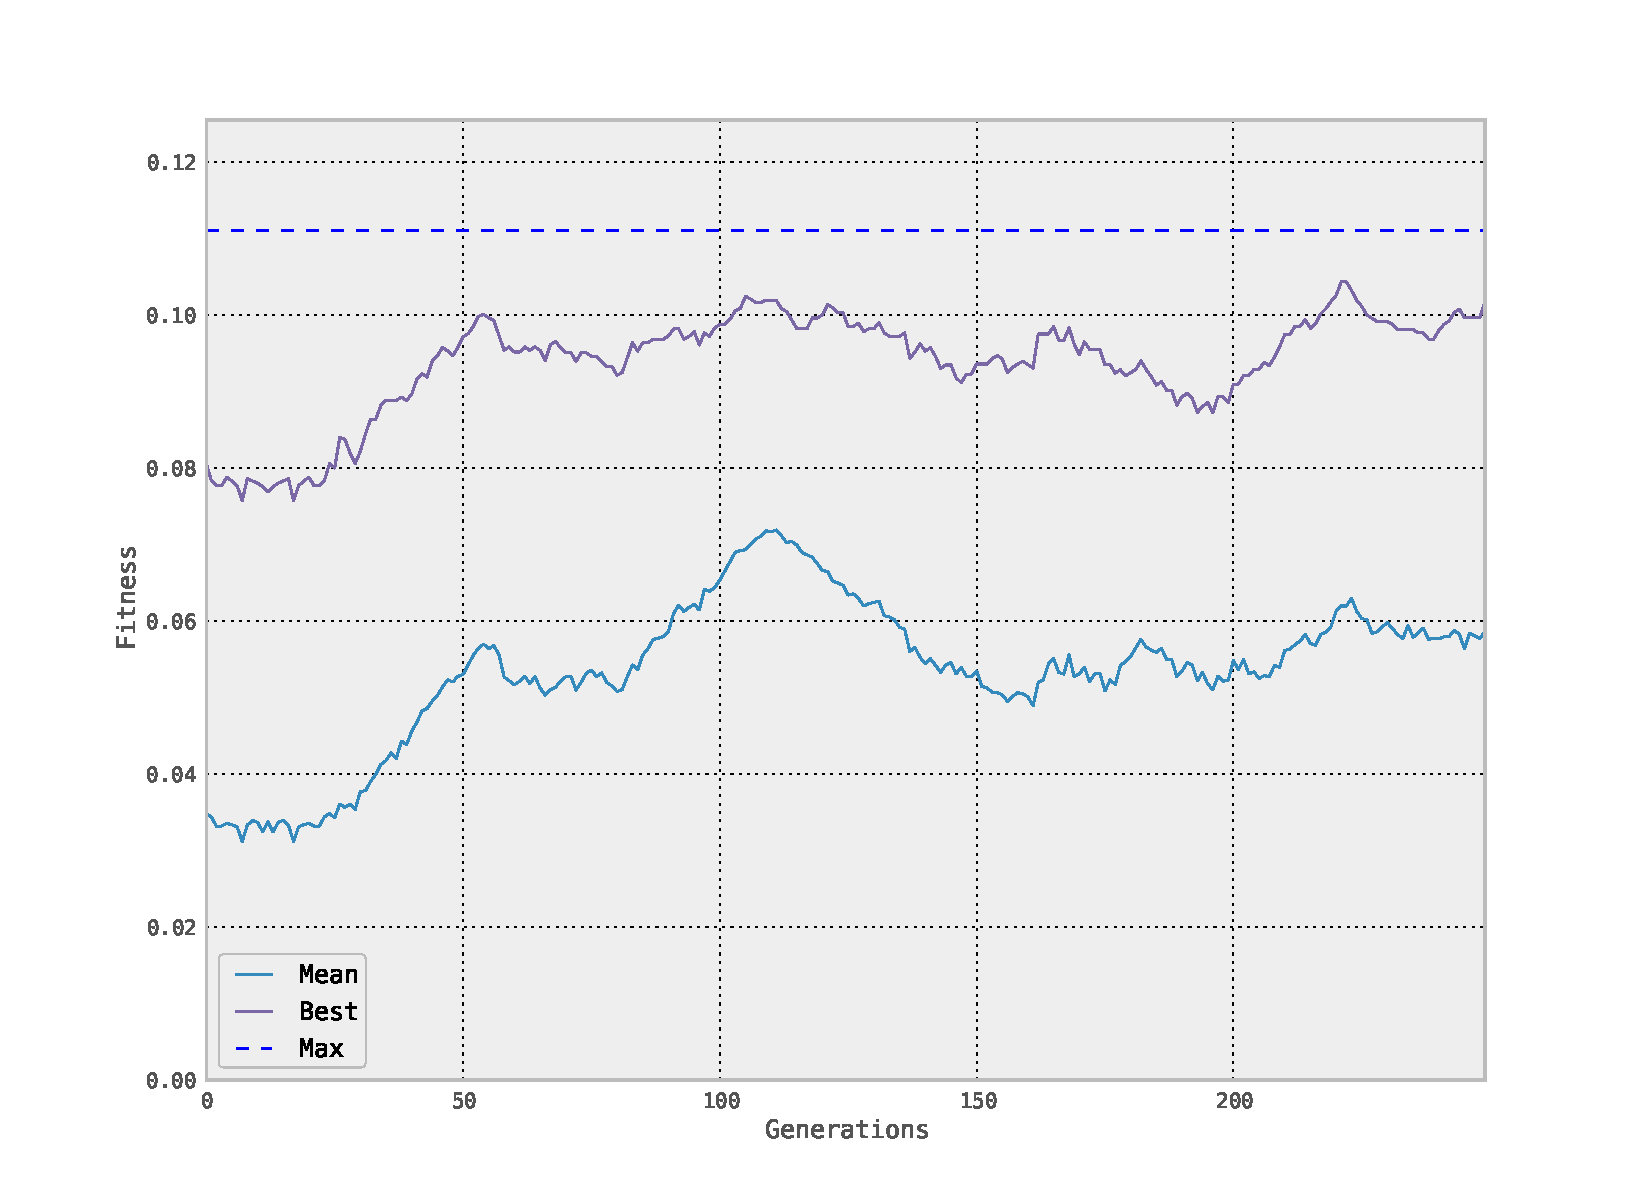
\includegraphics[scale =0.4] {images/section2/experimenta/fitness_5.pdf}
	\label{fig:subfig11}
}
\subfigure[Pheromones per edge]{
	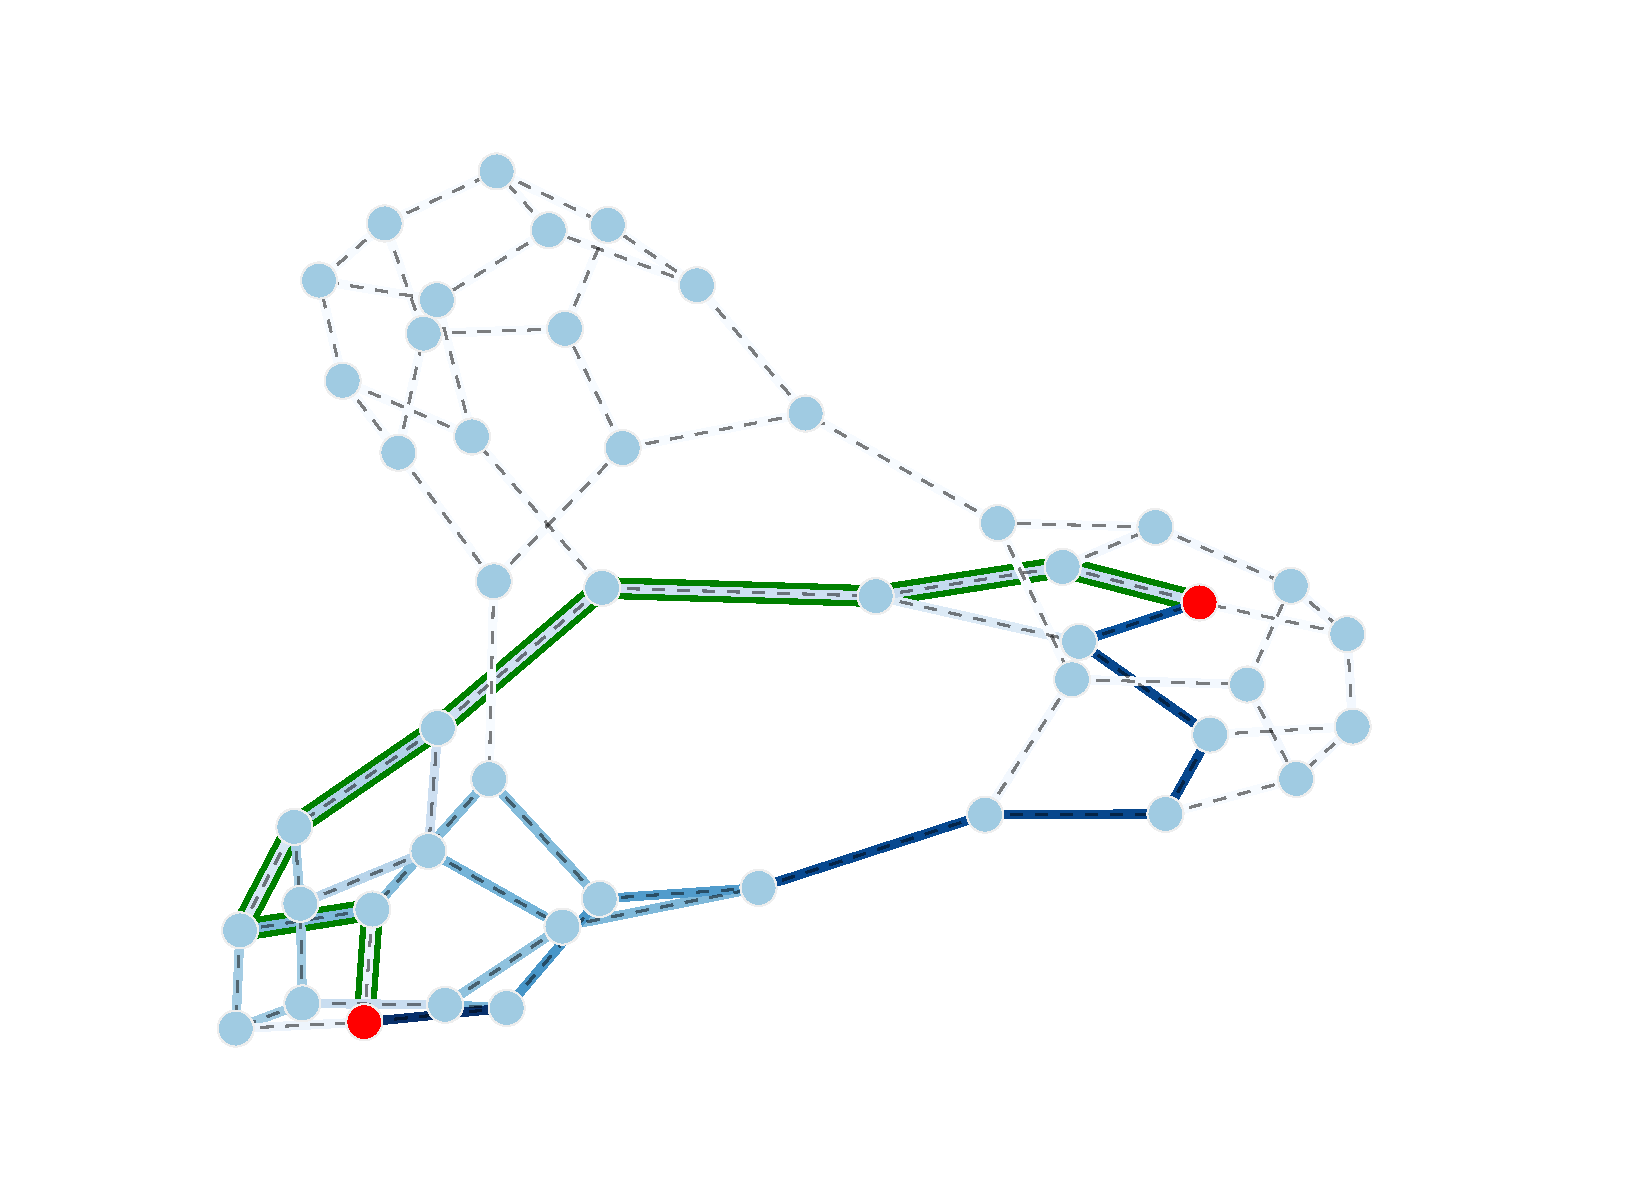
\includegraphics[scale =0.4] {images/section2/experimenta/pheromones_5_.pdf}
	\label{fig:subfig12}
}
%\caption[Optional caption for list of figures]{Caption of subfigures \subref{fig:subfig1}, \subref{fig:subfig2}}
\label{fig:fig1}
\end{figure}


\newpage
\subsubsection{Ant-like I, $k=10$}

\begin{figure}[ht]
\centering
\subfigure[Fitness evolution]{
	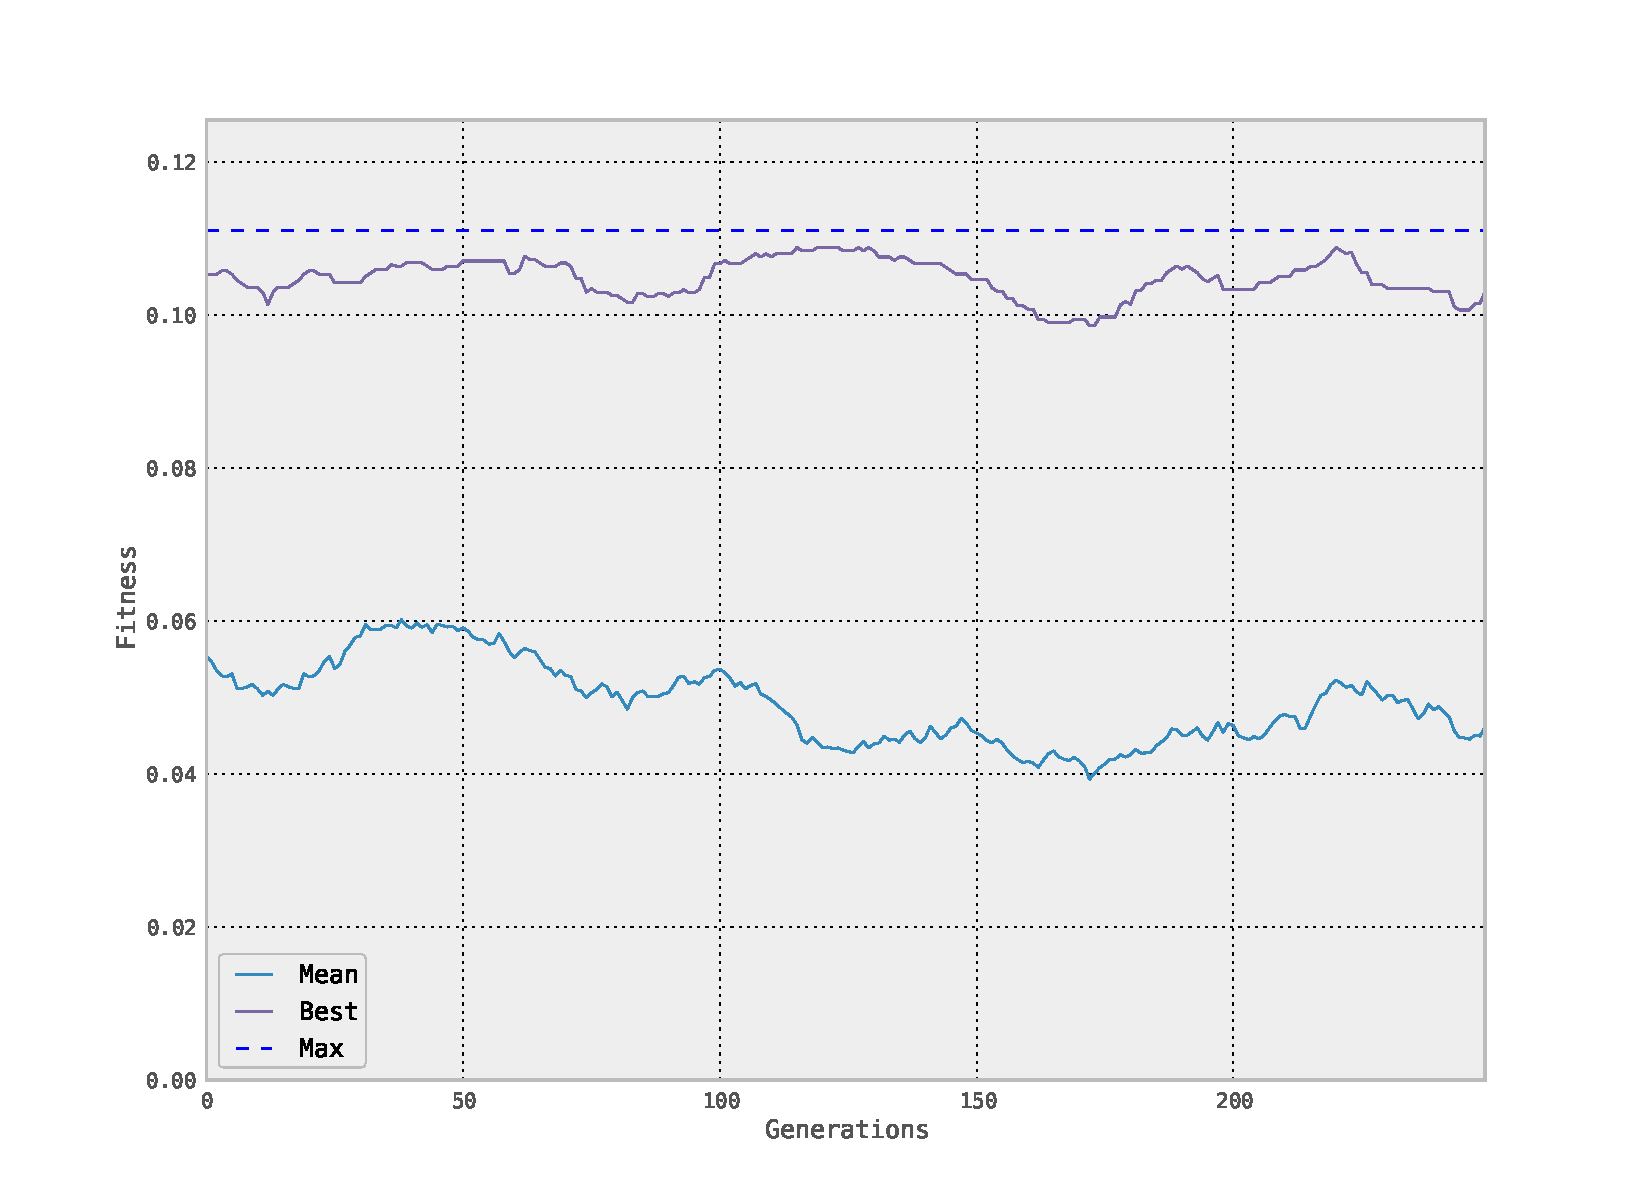
\includegraphics[scale =0.4] {images/section2/experimenta/fitness_10.pdf}
	\label{fig:subfig11}
}
\subfigure[Pheromones per edge]{
	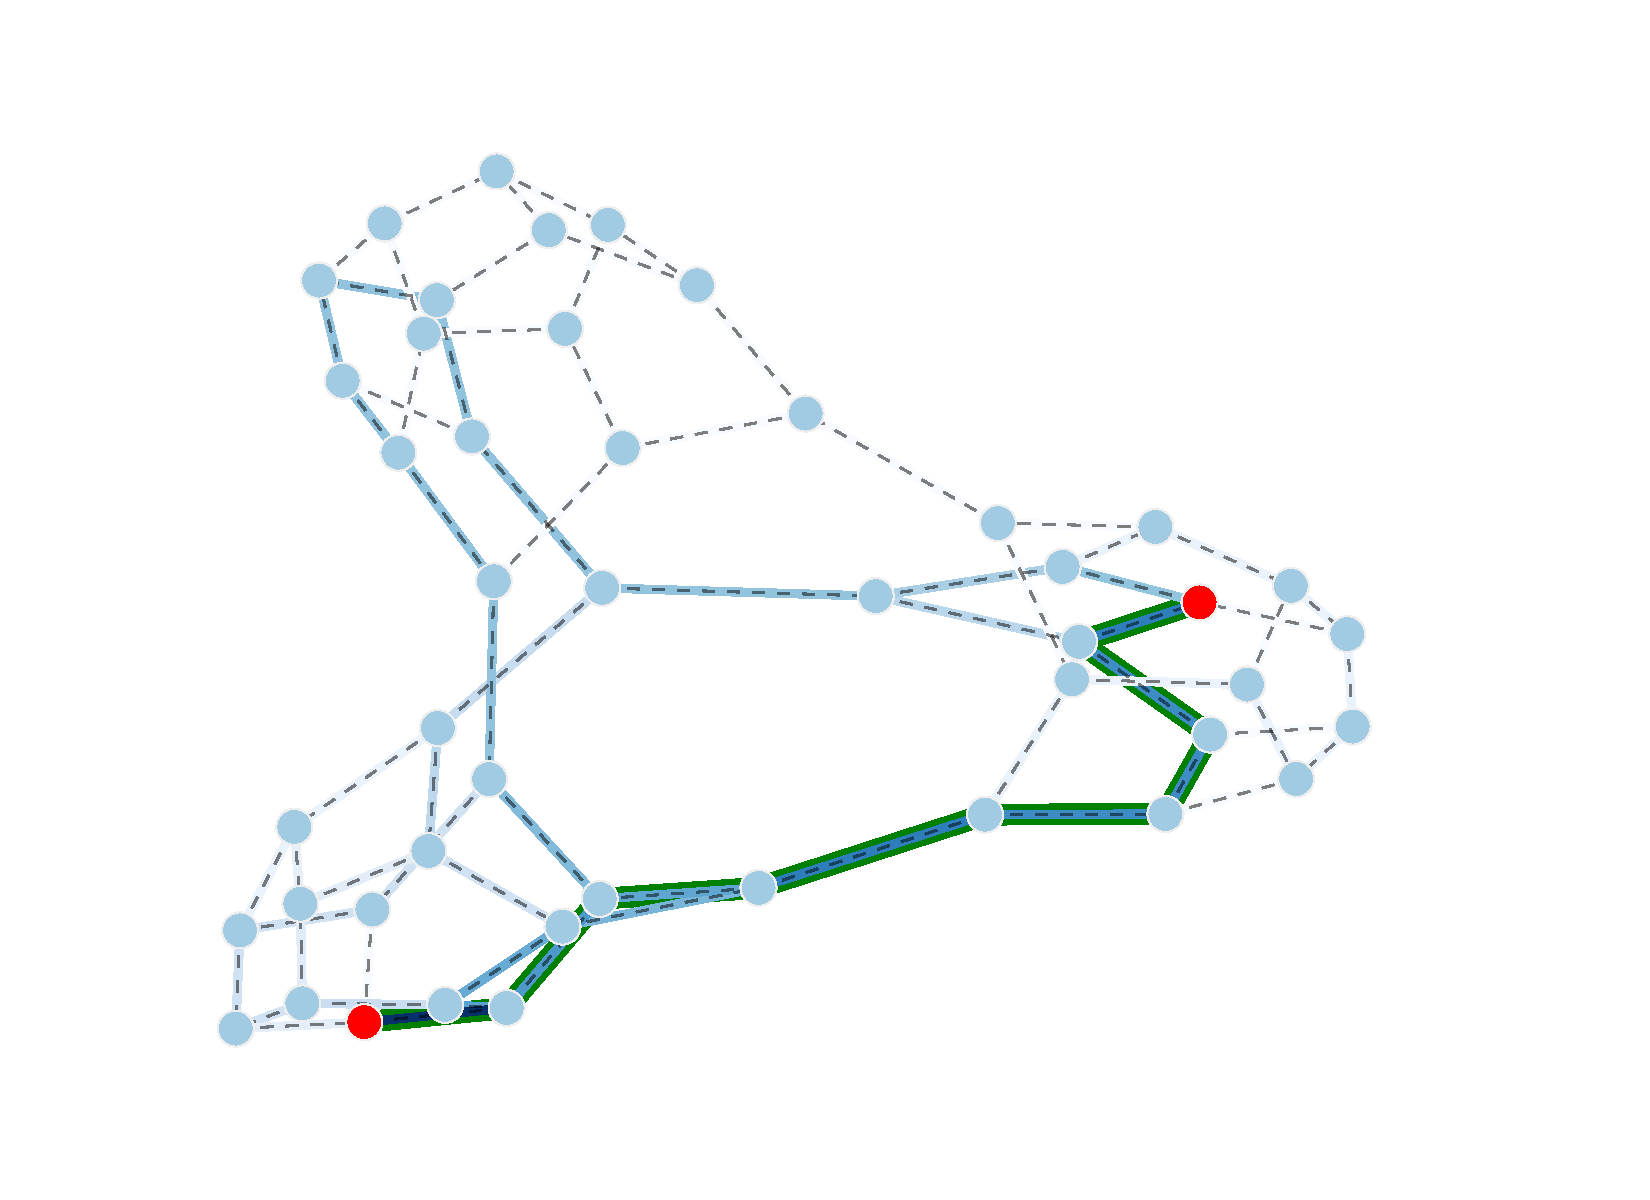
\includegraphics[scale =0.4] {images/section2/experimenta/pheromones_10_.pdf}
	\label{fig:subfig12}
}
%\caption[Optional caption for list of figures]{Caption of subfigures \subref{fig:subfig1}, \subref{fig:subfig2}}
\label{fig:fig1}
\end{figure}


\newpage
\subsubsection{Ant-like I, $k=15$}

\begin{figure}[ht]
\centering
\subfigure[Fitness evolution]{
	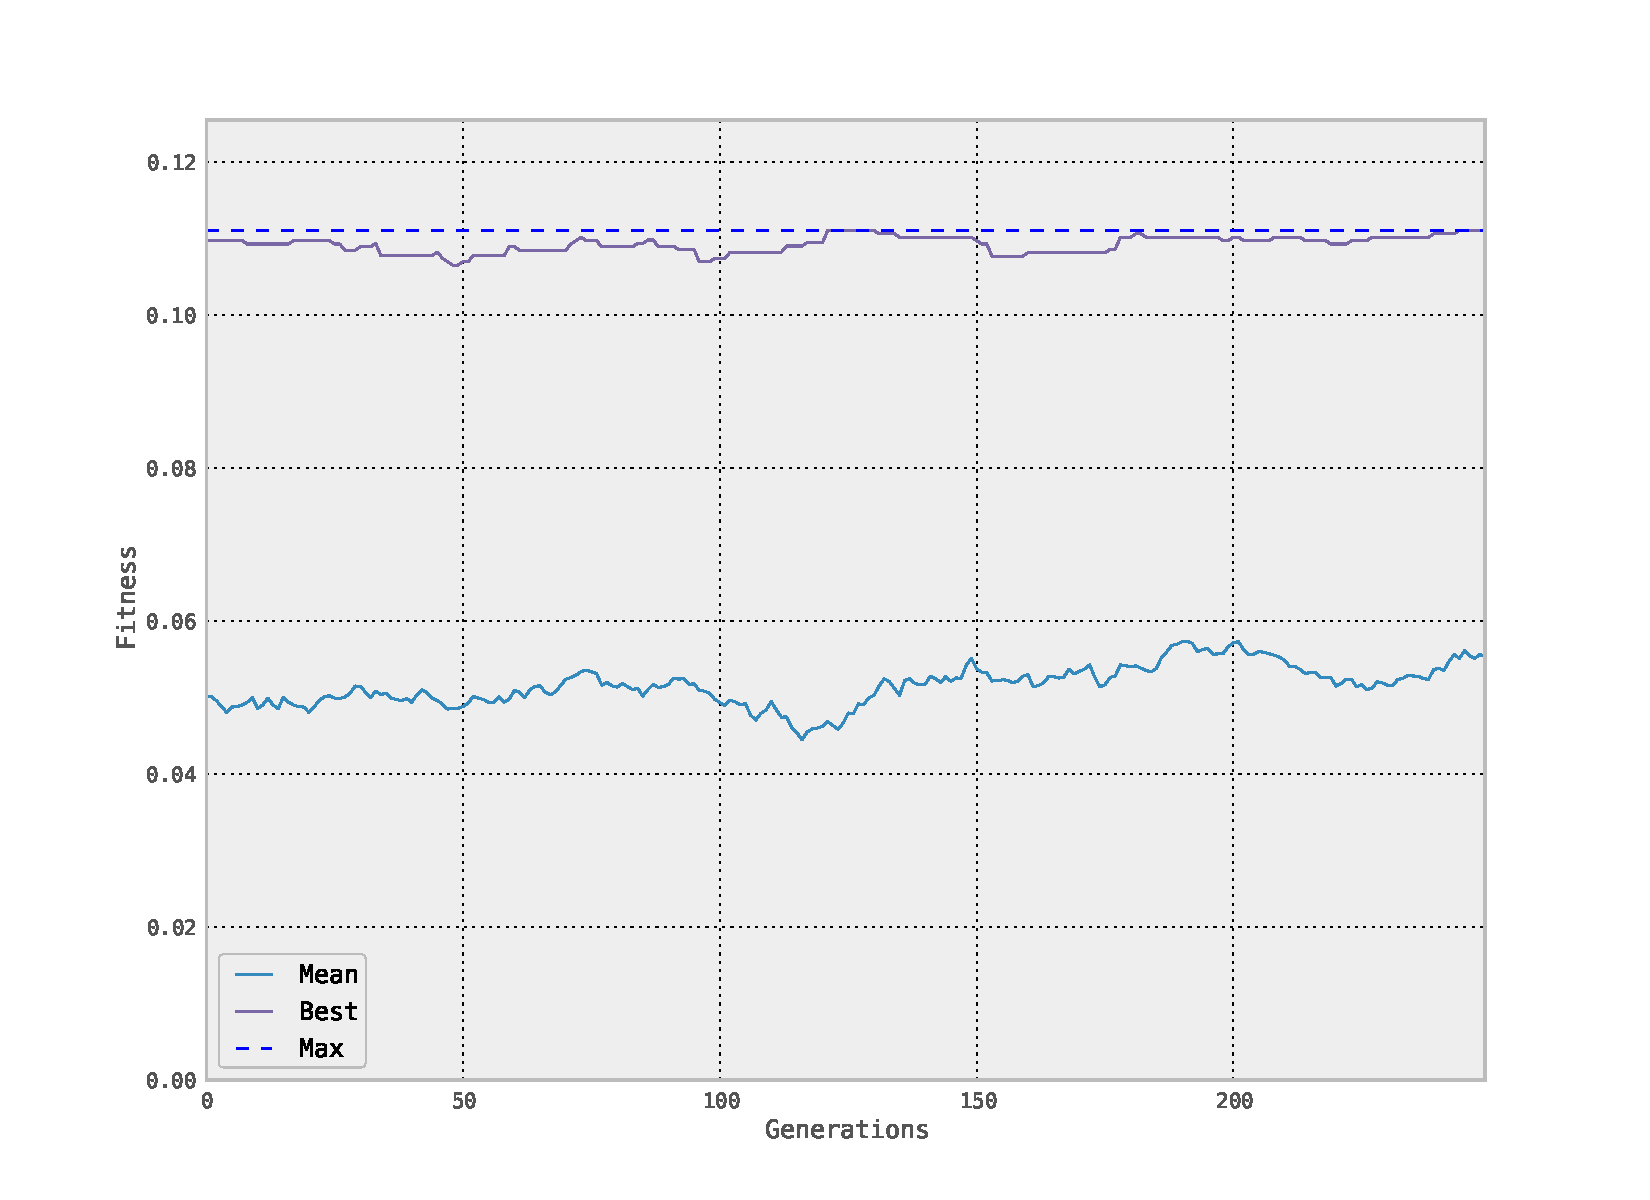
\includegraphics[scale =0.4] {images/section2/experimenta/fitness_15.pdf}
	\label{fig:subfig11}
}
\subfigure[Pheromones per edge]{
	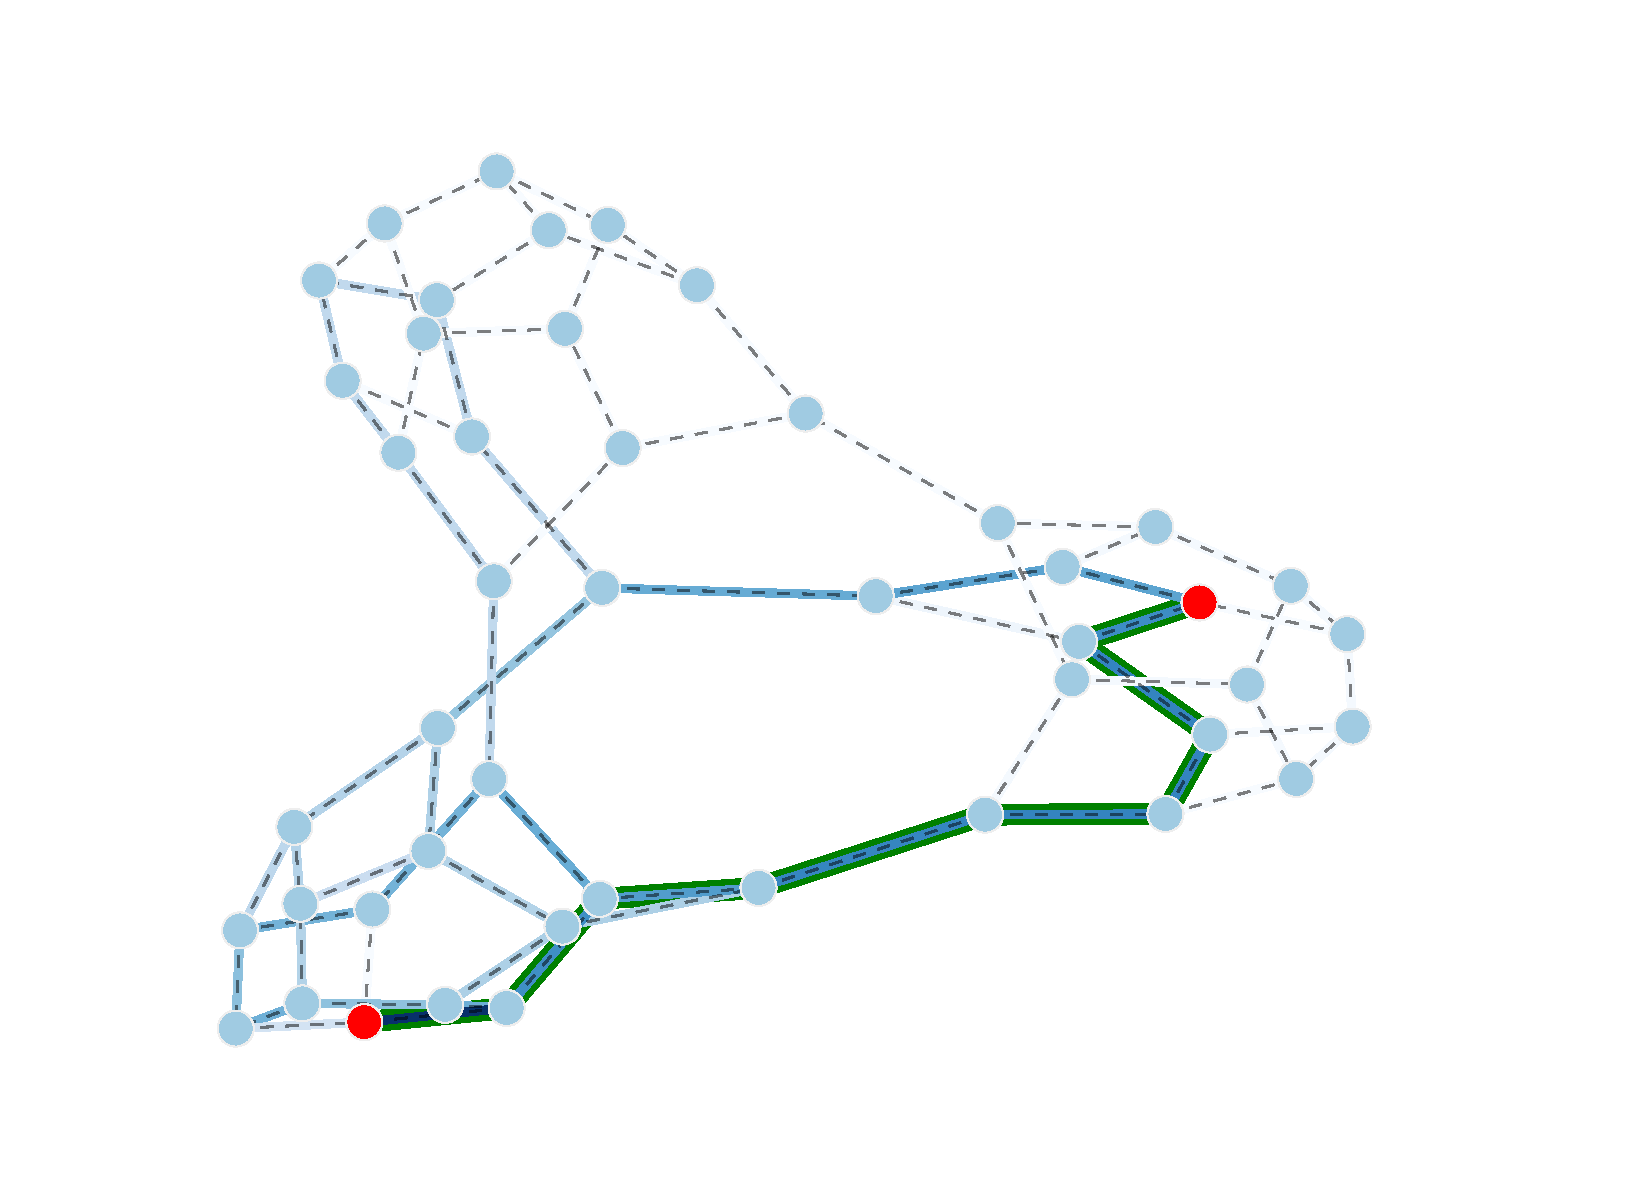
\includegraphics[scale =0.4] {images/section2/experimenta/pheromones_15_.pdf}
	\label{fig:subfig12}
}
%\caption[Optional caption for list of figures]{Caption of subfigures \subref{fig:subfig1}, \subref{fig:subfig2}}
\label{fig:fig1}
\end{figure}

\newpage
\subsubsection{Ant-like I, $k=50$}

\begin{figure}[ht]
\centering
\subfigure[Fitness evolution]{
	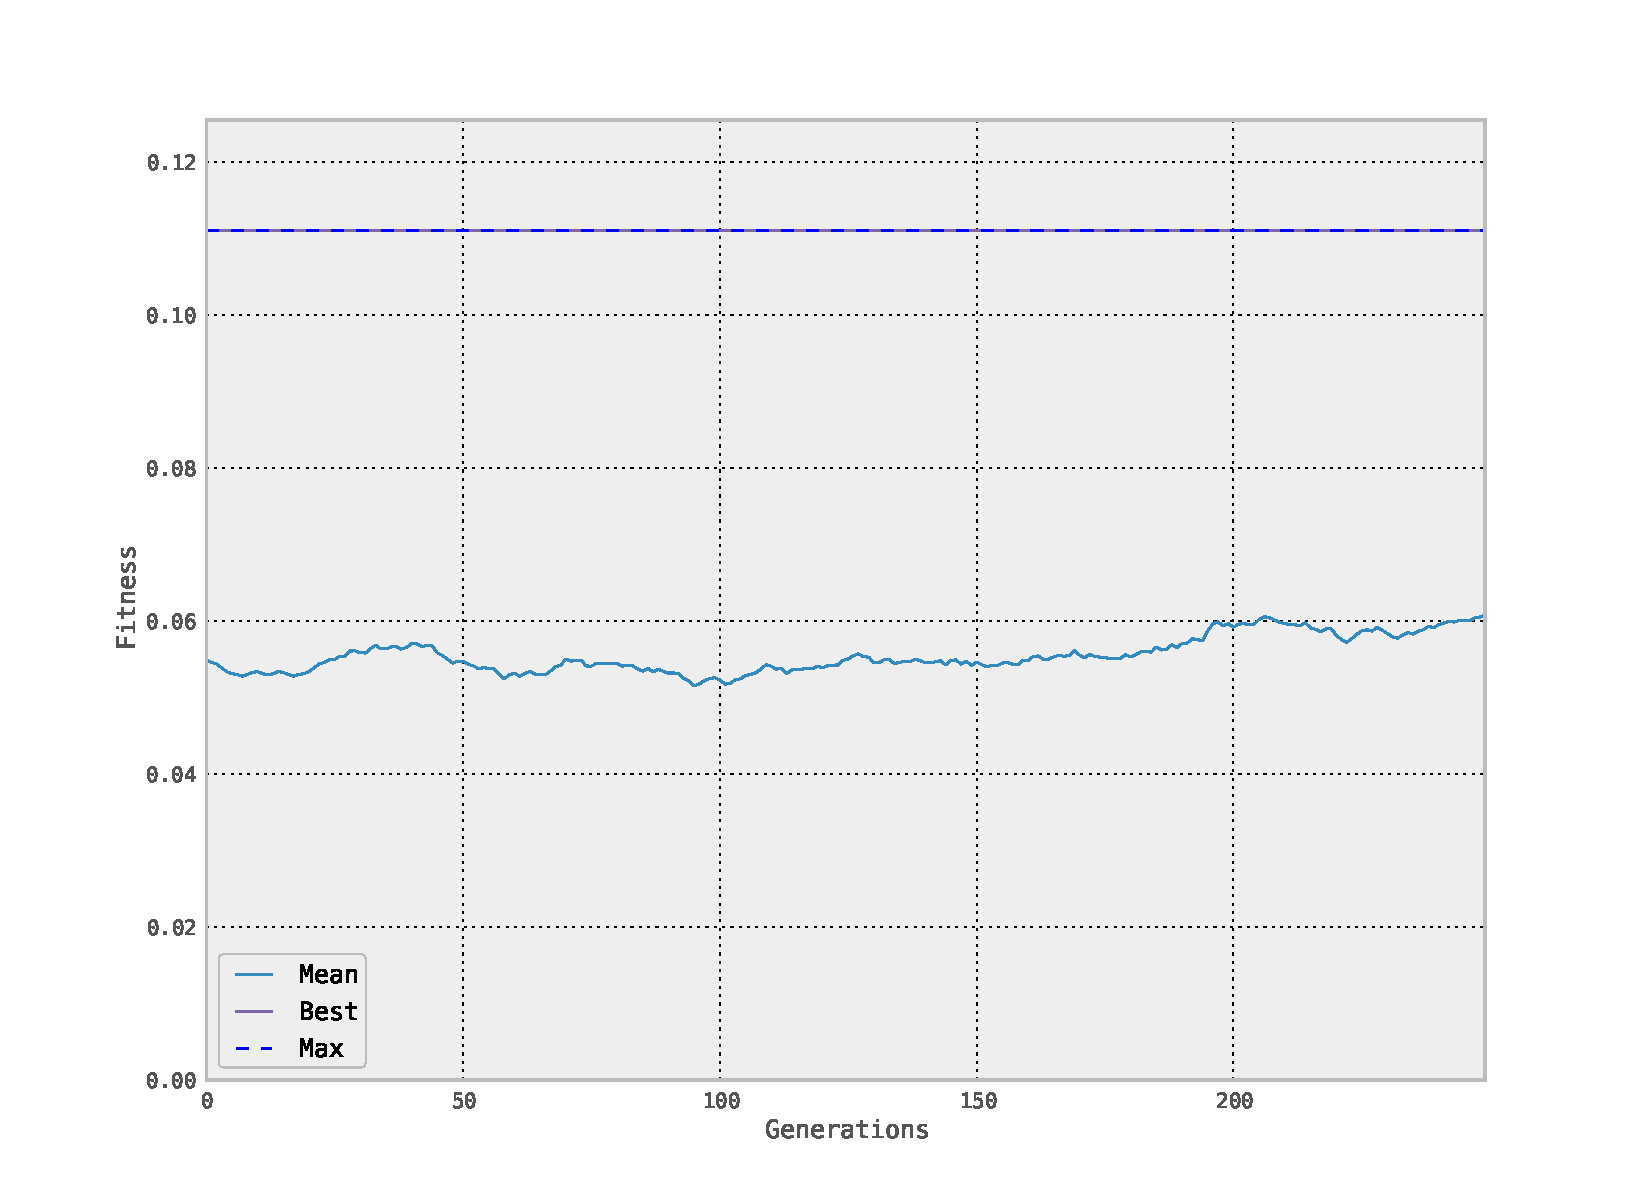
\includegraphics[scale =0.4] {images/section2/experimenta/fitness_50.pdf}
	\label{fig:subfig11}
}
\subfigure[Pheromones per edge]{
	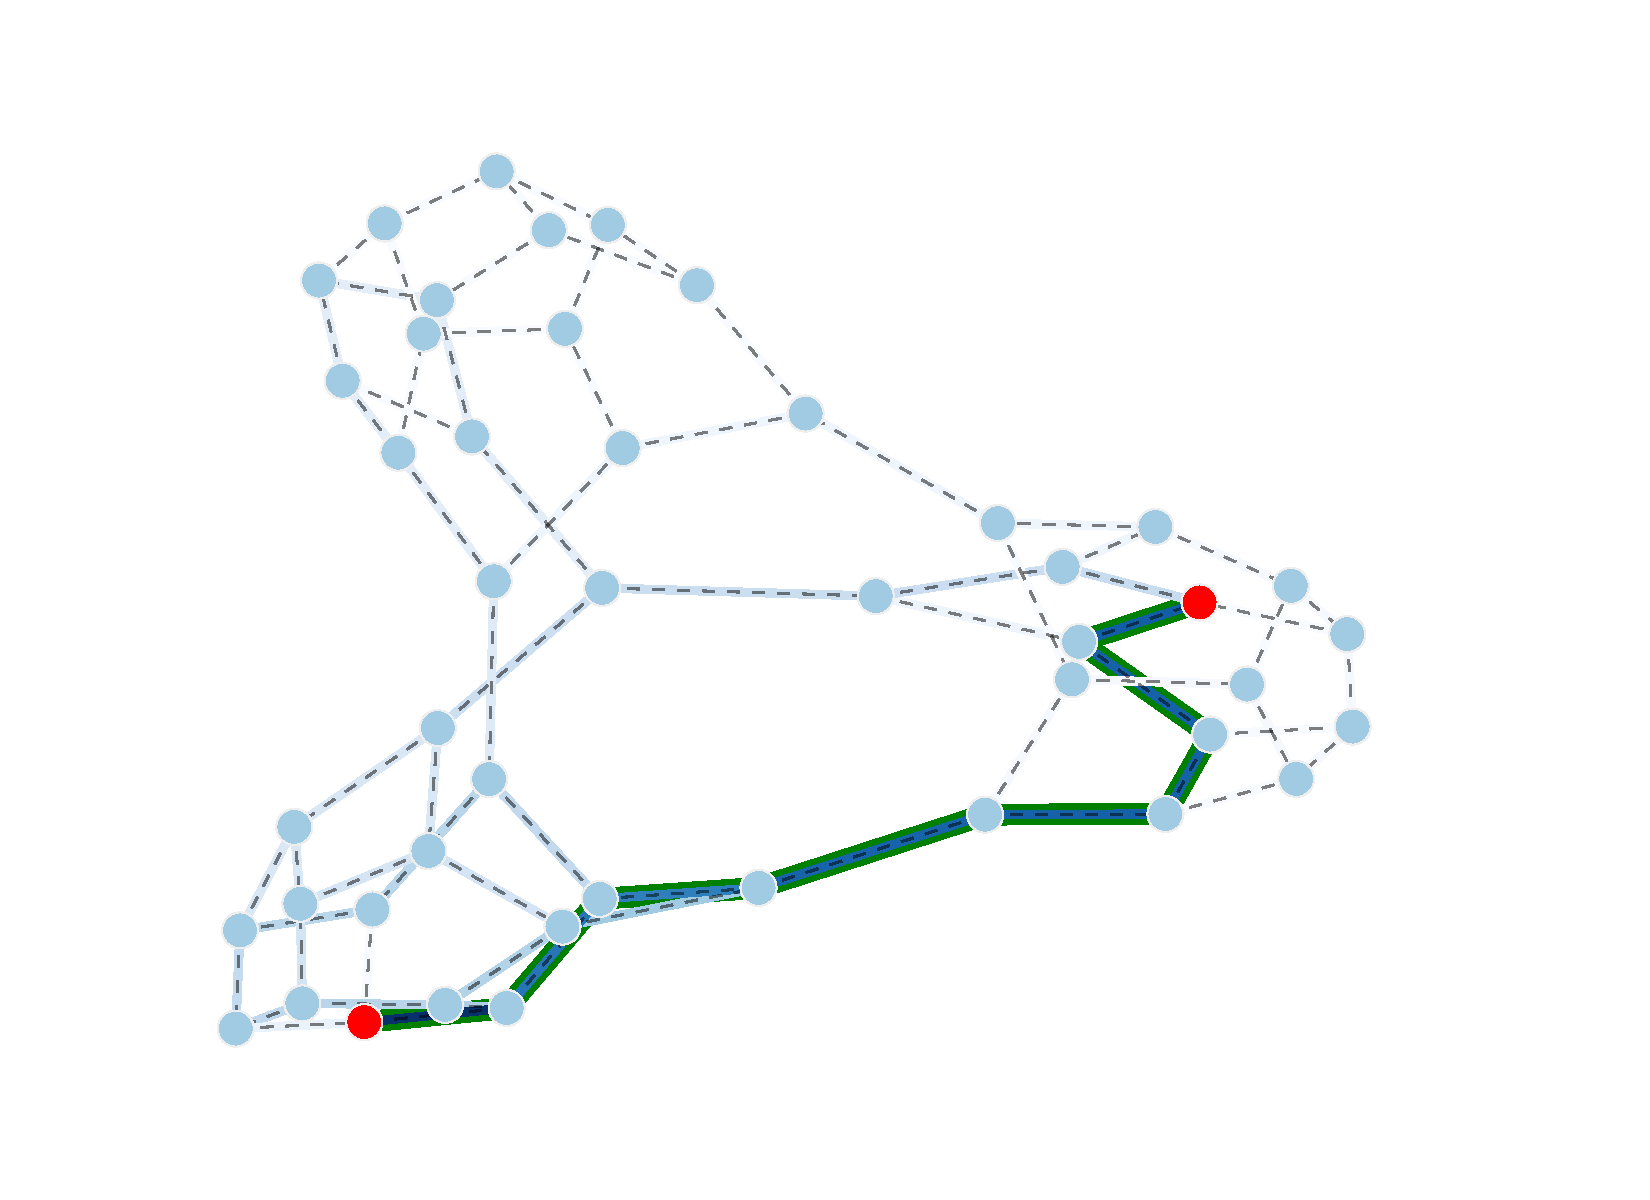
\includegraphics[scale =0.4] {images/section2/experimenta/pheromones_50_.pdf}
	\label{fig:subfig12}
}
%\caption[Optional caption for list of figures]{Caption of subfigures \subref{fig:subfig1}, \subref{fig:subfig2}}
\label{fig:fig1}
\end{figure}


\newpage
\subsubsection{Ant-like I, $k=100$}

\begin{figure}[ht]
\centering
\subfigure[Fitness evolution]{
	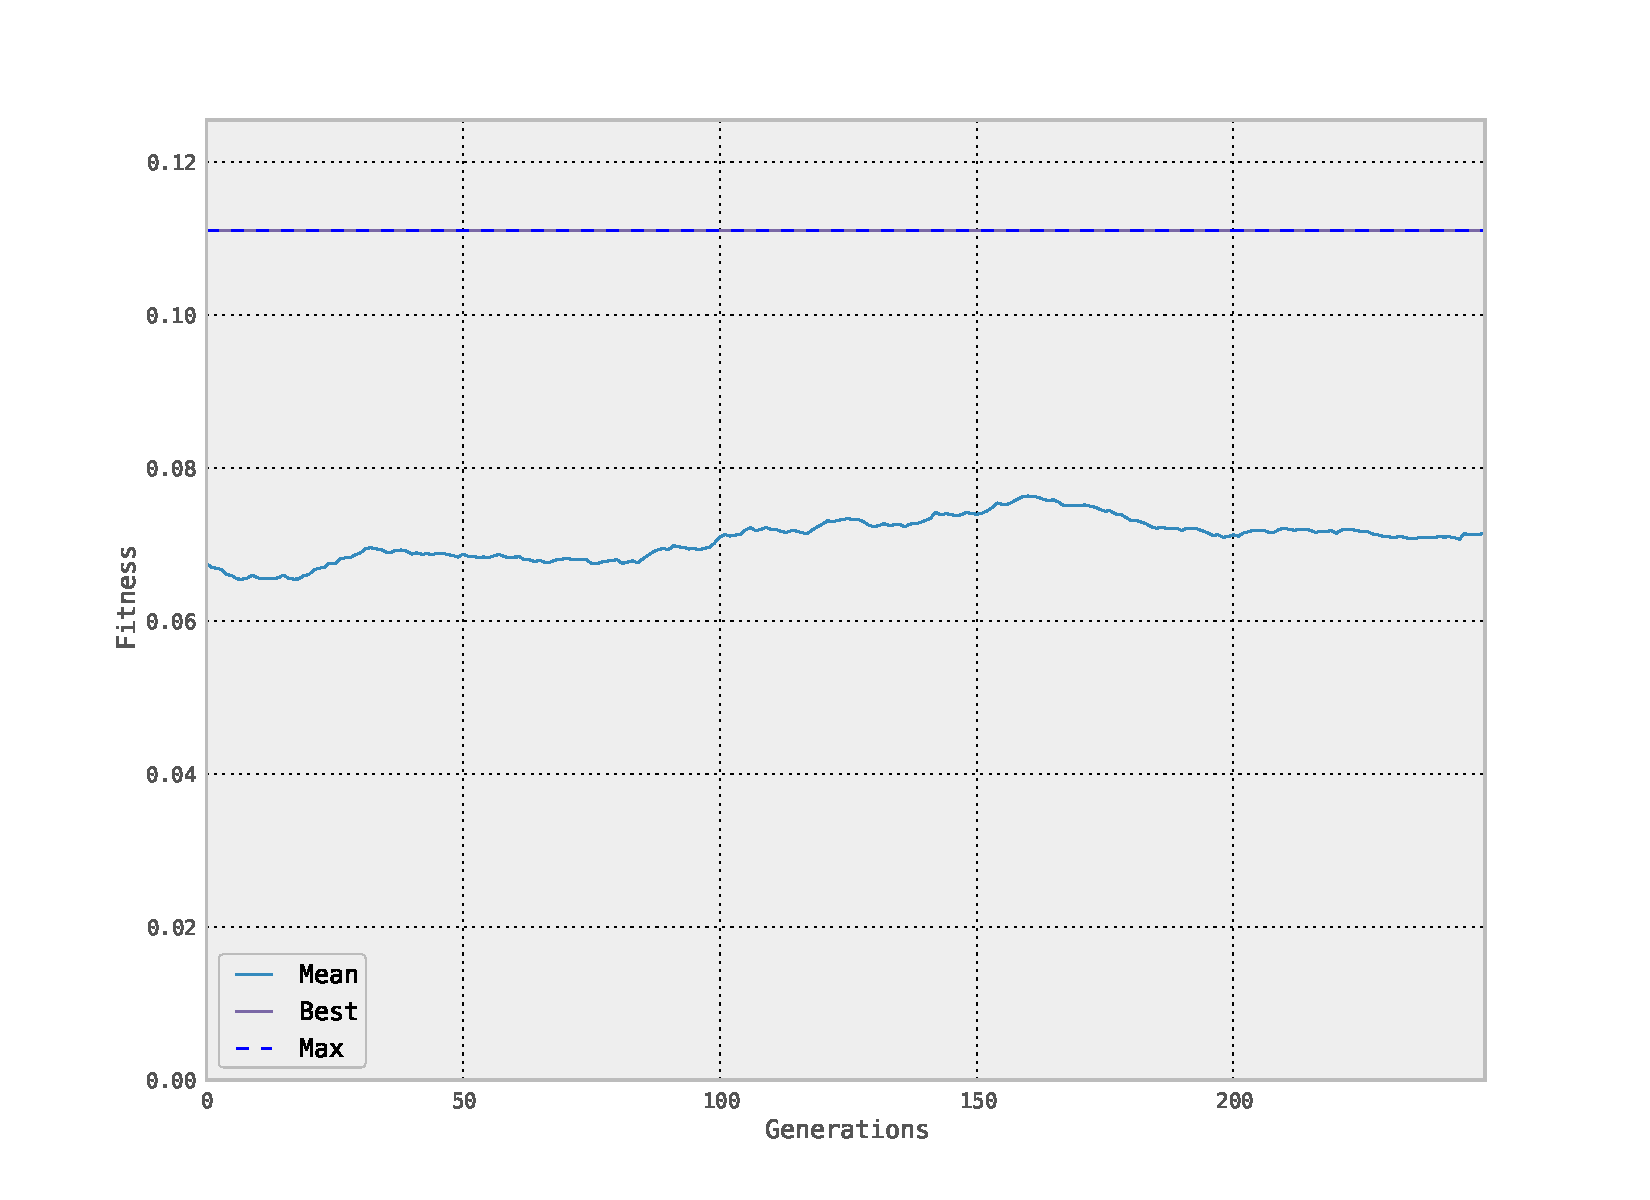
\includegraphics[scale =0.4] {images/section2/experimenta/fitness_100.pdf}
	\label{fig:subfig11}
}
\subfigure[Pheromones per edge]{
	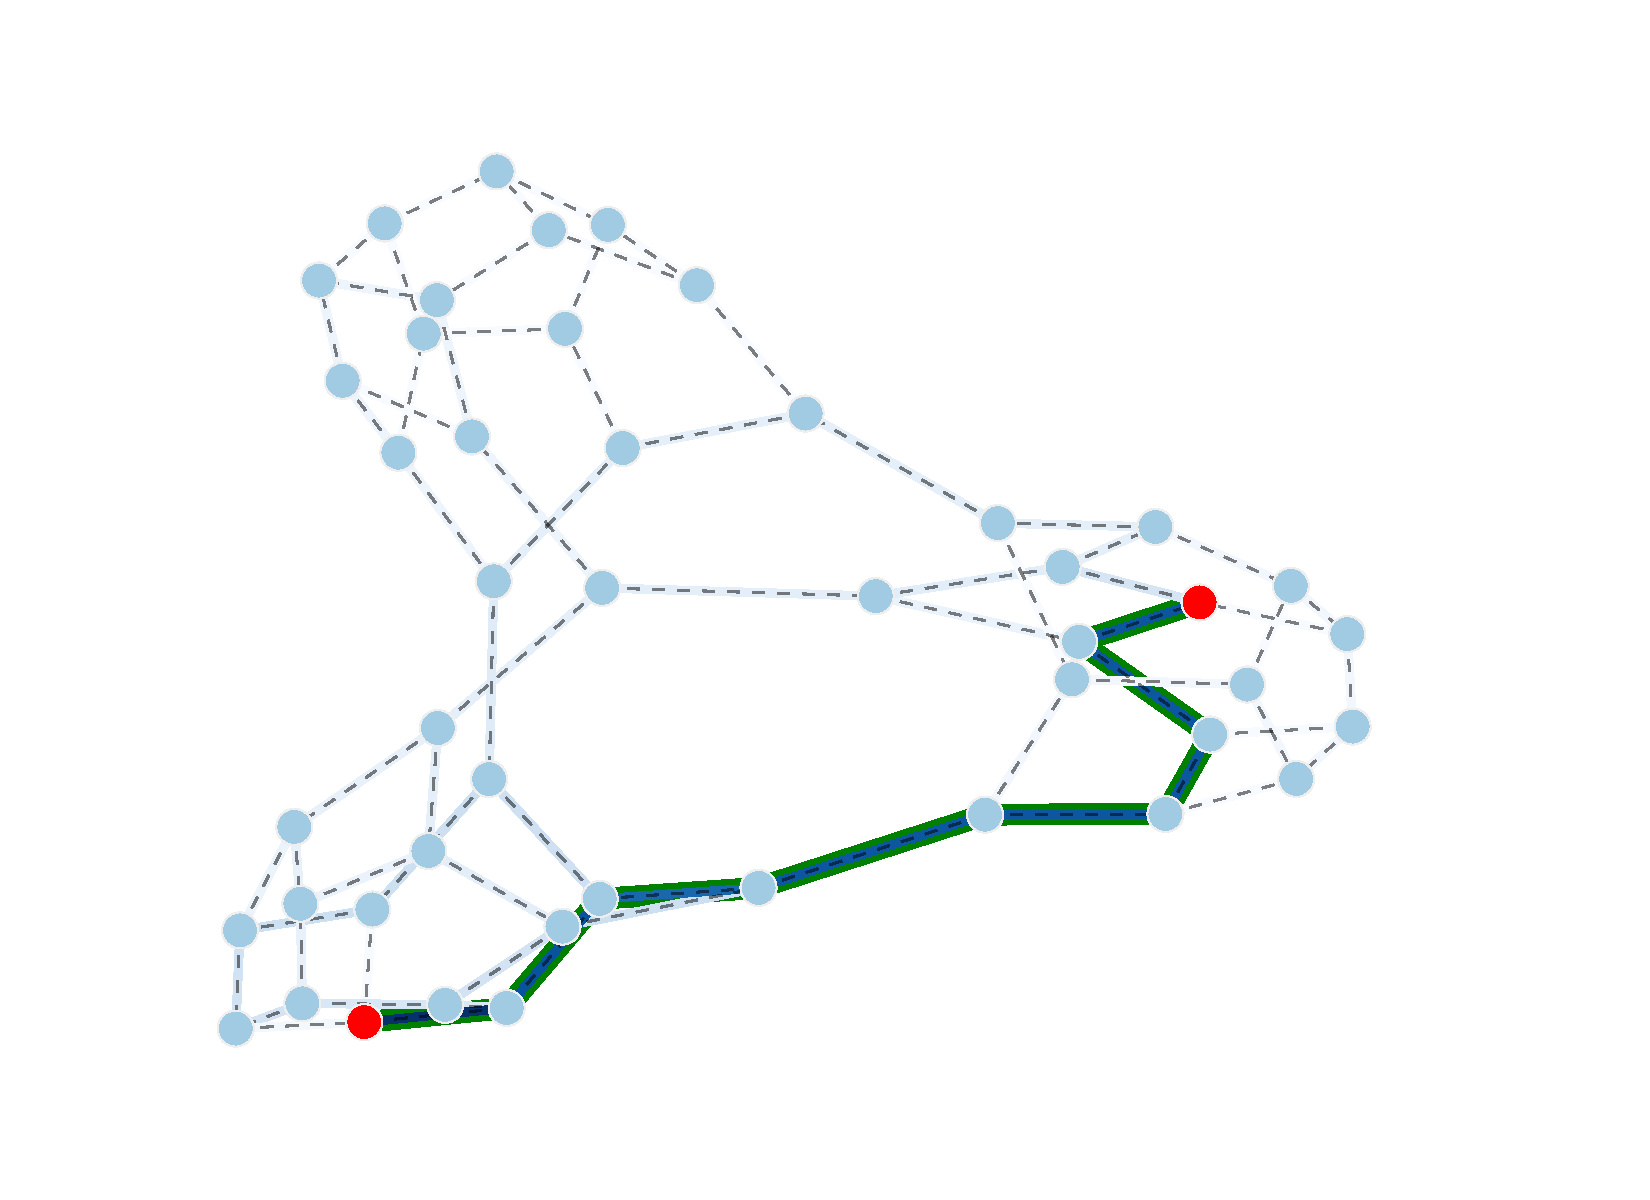
\includegraphics[scale =0.4] {images/section2/experimenta/pheromones_100_.pdf}
	\label{fig:subfig12}
}
%\caption[Optional caption for list of figures]{Caption of subfigures \subref{fig:subfig1}, \subref{fig:subfig2}}
\label{fig:fig1}
\end{figure}










\newpage
\subsubsection{Ant-like II, $k=5$}

\begin{figure}[ht]
\centering
\subfigure[Fitness evolution]{
	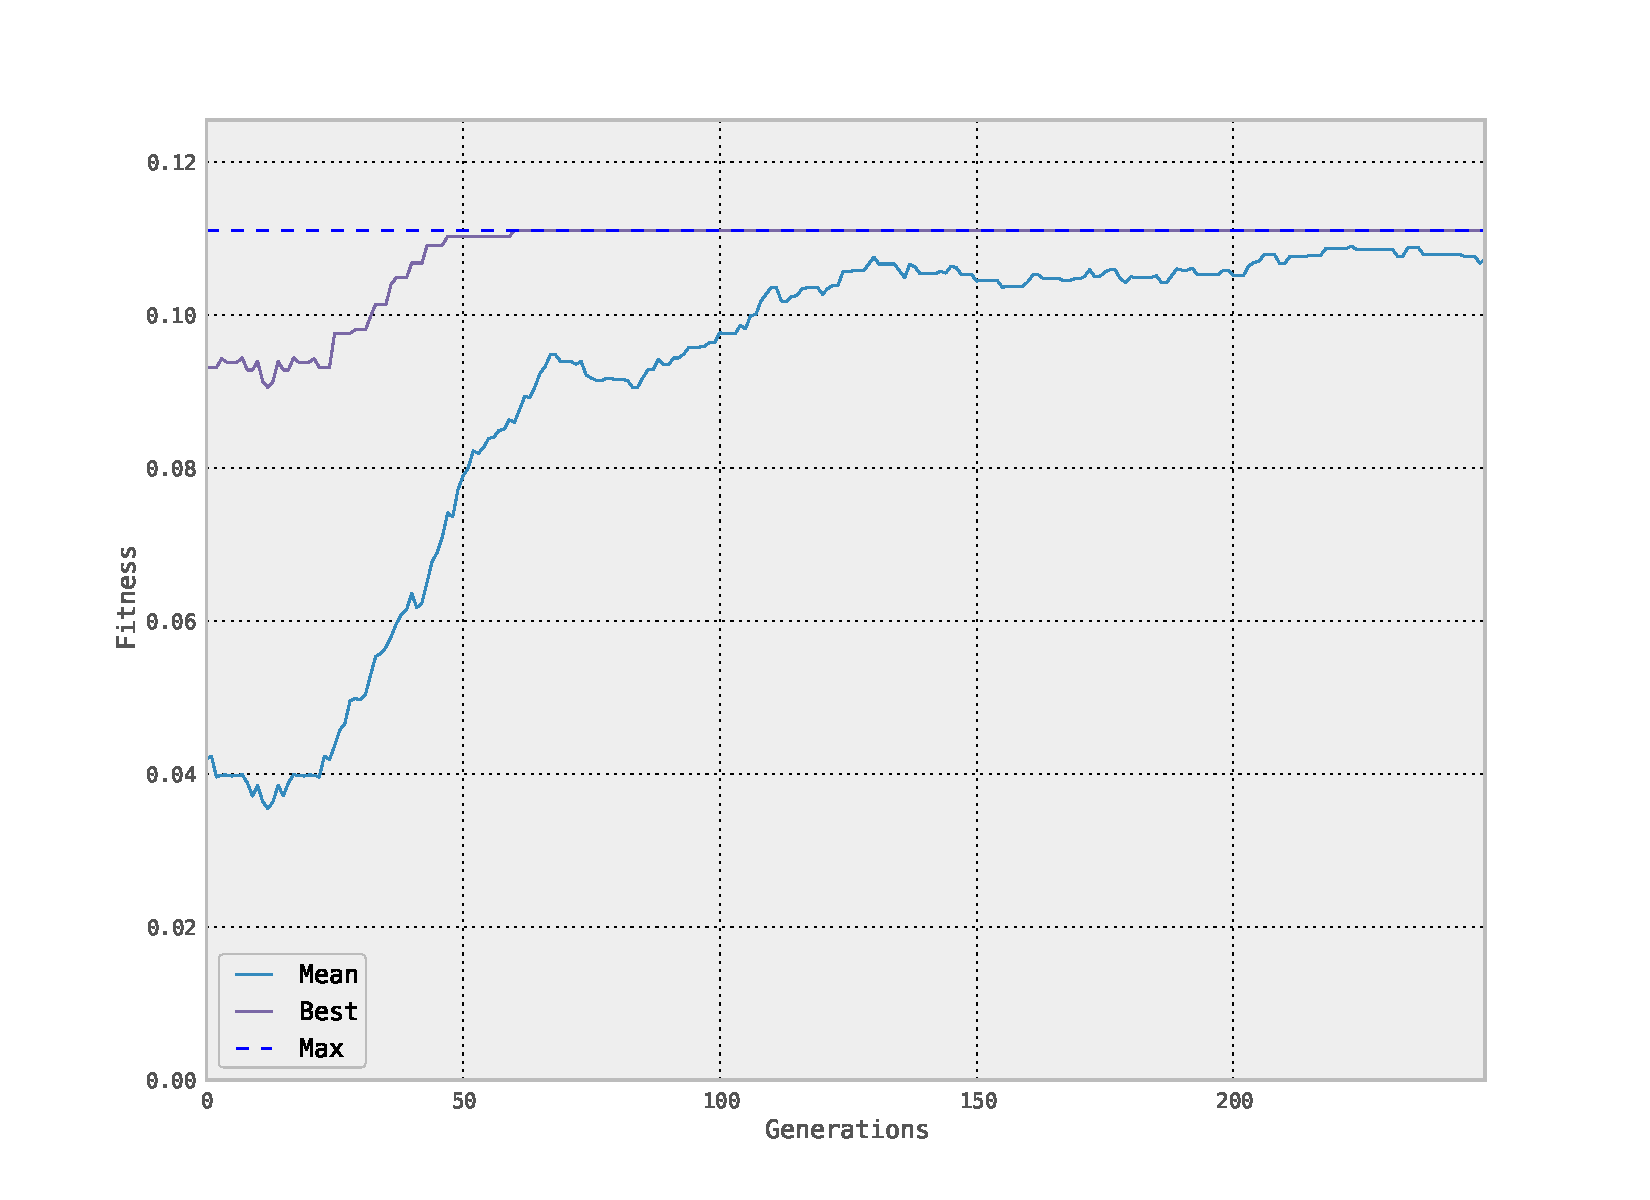
\includegraphics[scale =0.4] {images/section2/experimentb/fitness_5.pdf}
	\label{fig:subfig11}
}
\subfigure[Pheromones per edge]{
	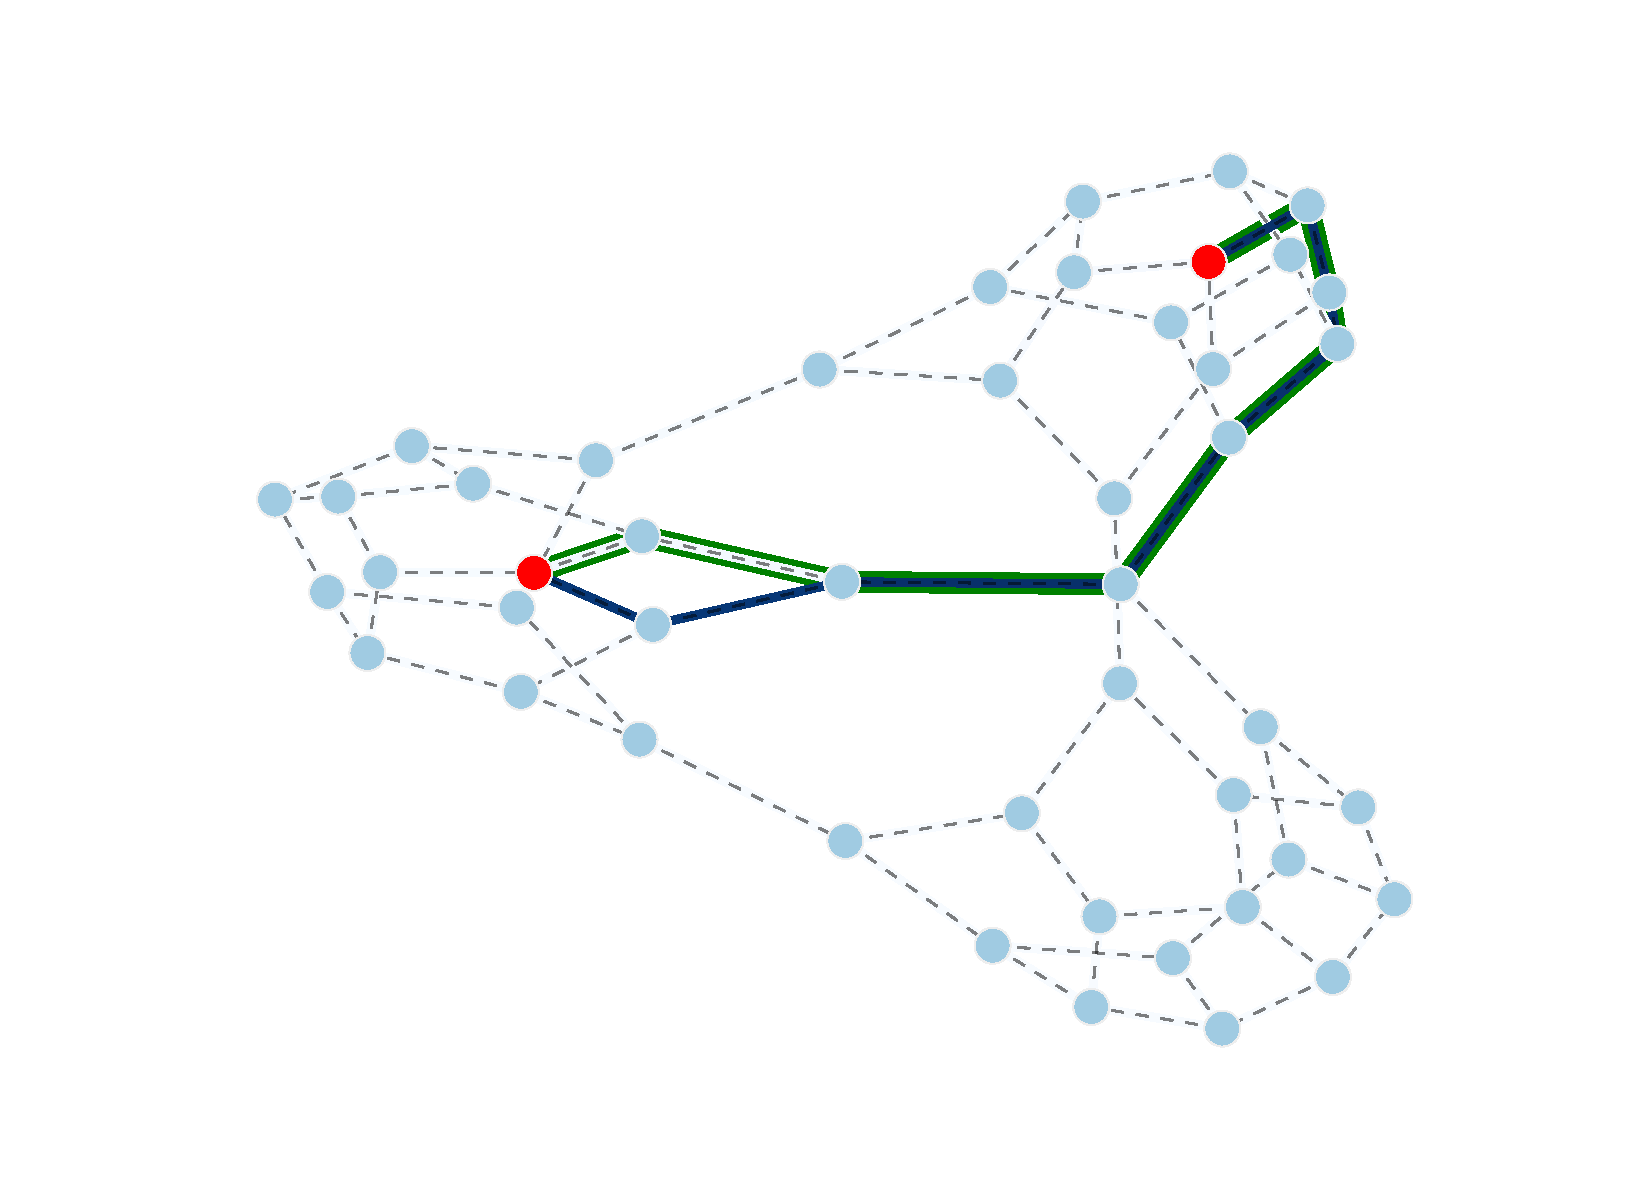
\includegraphics[scale =0.4] {images/section2/experimentb/pheromones_5_.pdf}
	\label{fig:subfig12}
}
%\caption[Optional caption for list of figures]{Caption of subfigures \subref{fig:subfig1}, \subref{fig:subfig2}}
\label{fig:fig1}
\end{figure}


\newpage
\subsubsection{Ant-like II, $k=10$}

\begin{figure}[ht]
\centering
\subfigure[Fitness evolution]{
	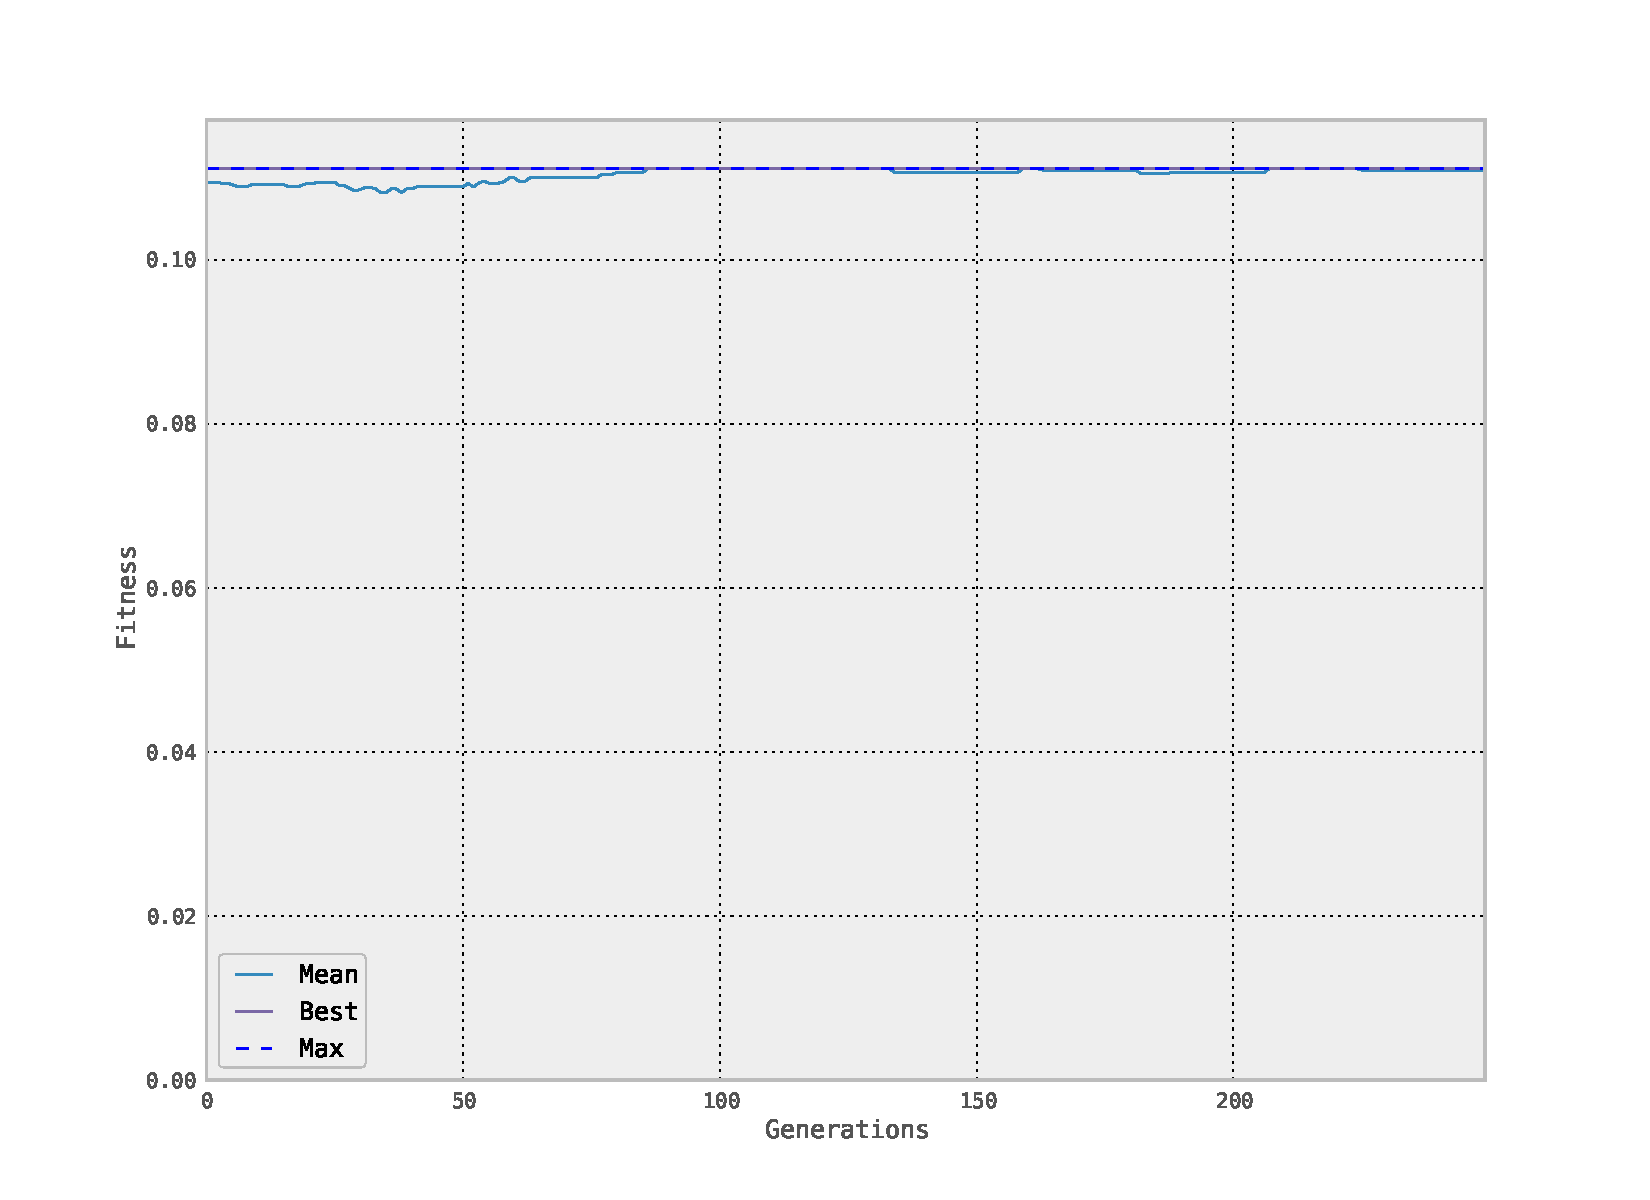
\includegraphics[scale =0.4] {images/section2/experimentb/fitness_10.pdf}
	\label{fig:subfig11}
}
\subfigure[Pheromones per edge]{
	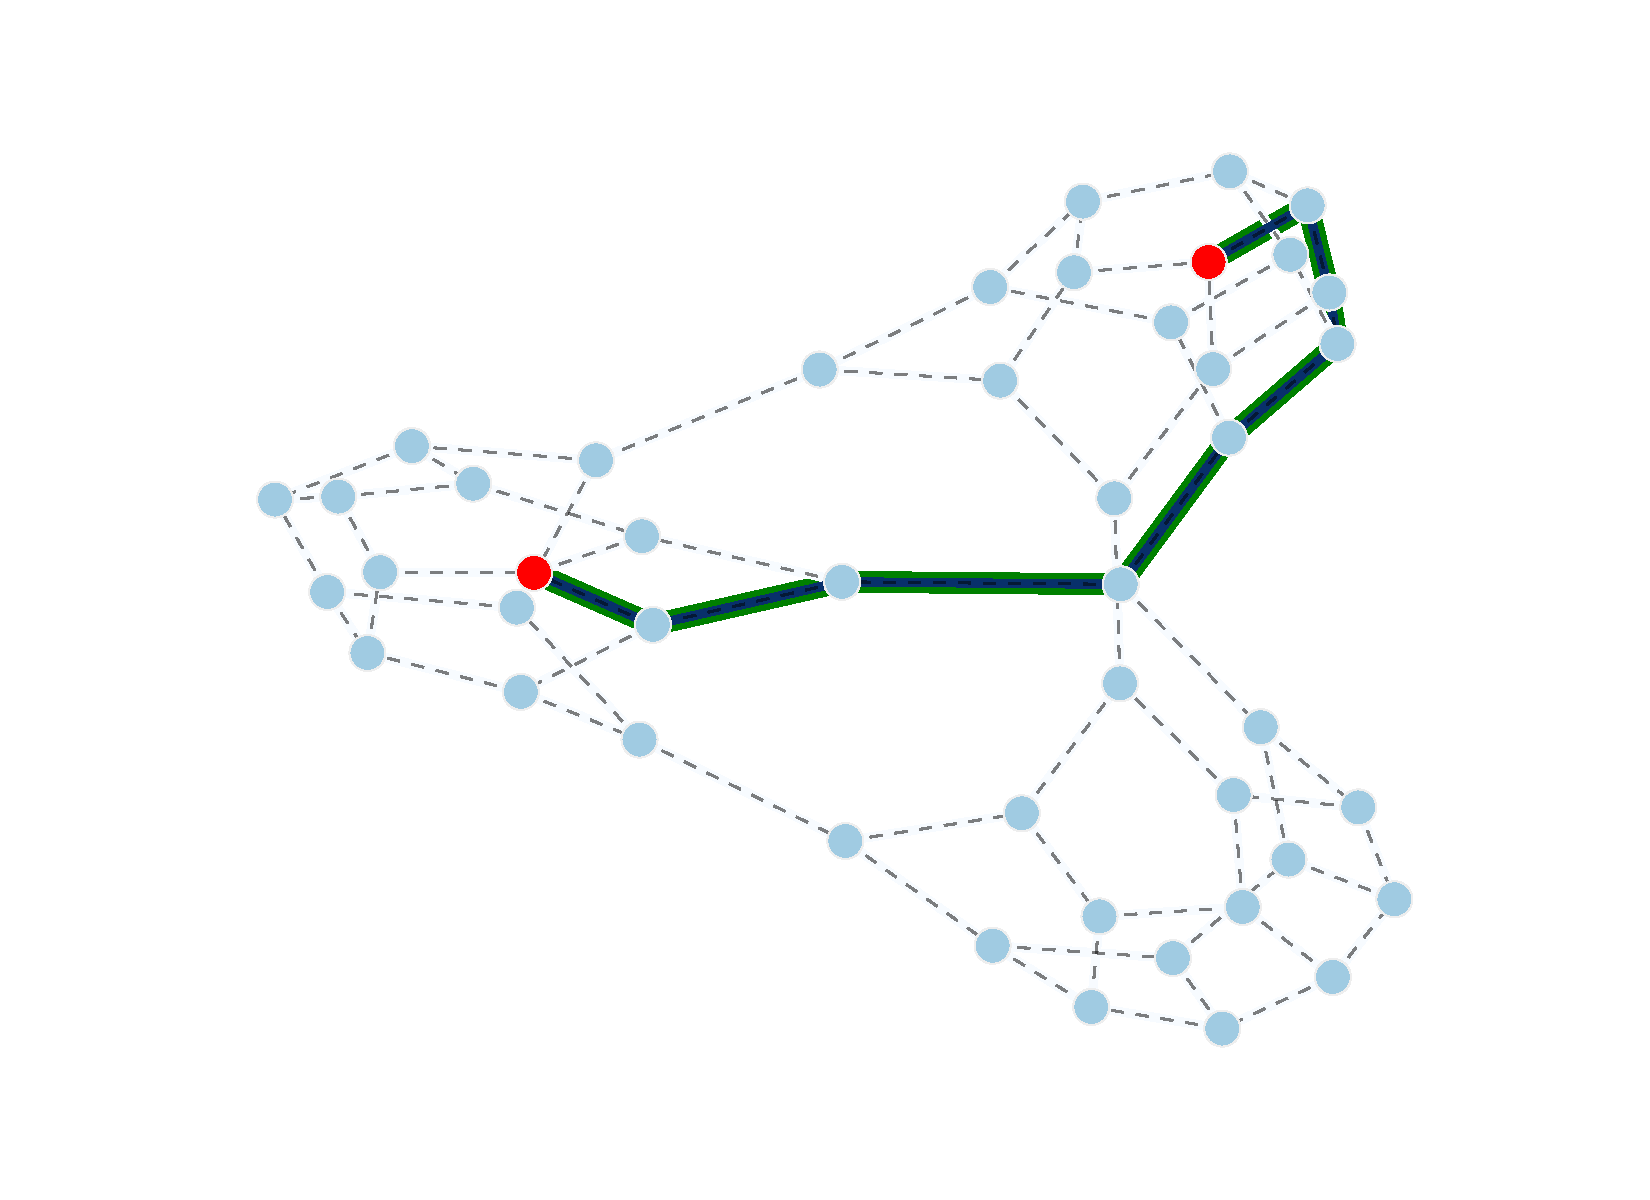
\includegraphics[scale =0.4] {images/section2/experimentb/pheromones_10_.pdf}
	\label{fig:subfig12}
}
%\caption[Optional caption for list of figures]{Caption of subfigures \subref{fig:subfig1}, \subref{fig:subfig2}}
\label{fig:fig1}
\end{figure}


\newpage
\subsubsection{Ant-like II, $k=15$}

\begin{figure}[ht]
\centering
\subfigure[Fitness evolution]{
	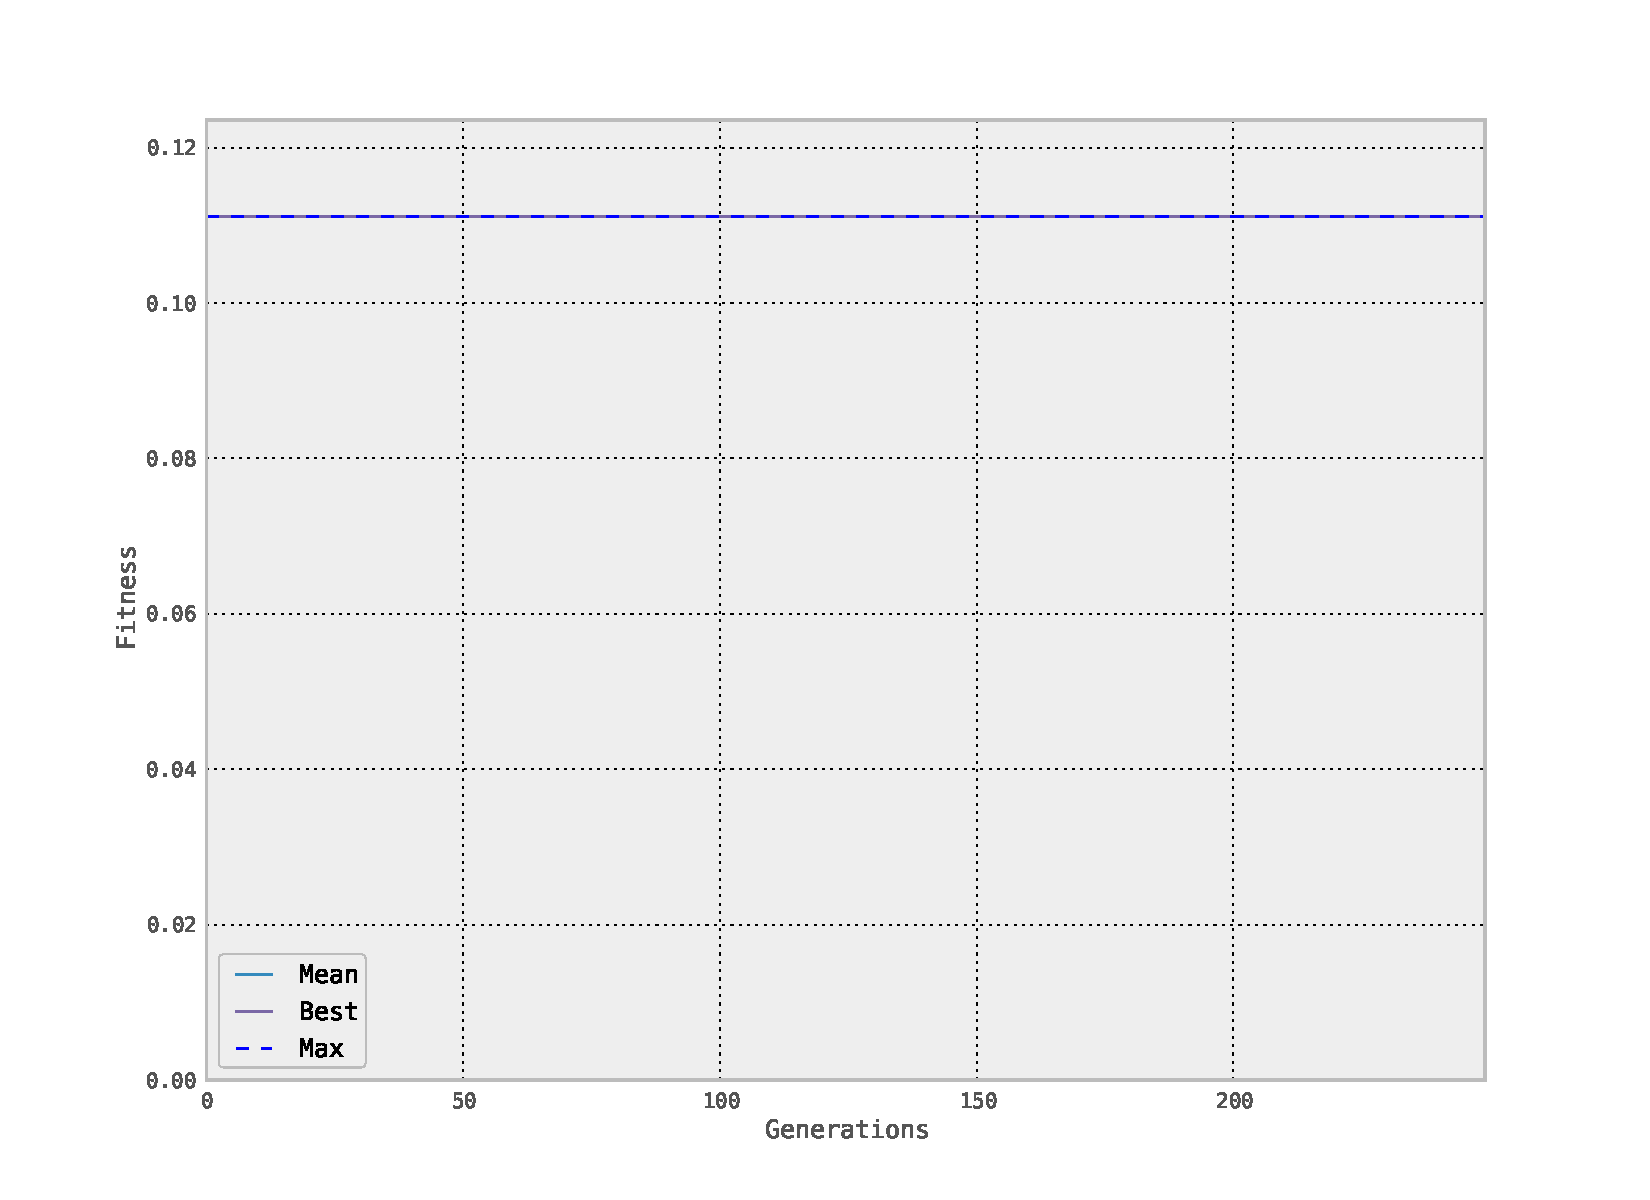
\includegraphics[scale =0.4] {images/section2/experimentb/fitness_15.pdf}
	\label{fig:subfig11}
}
\subfigure[Pheromones per edge]{
	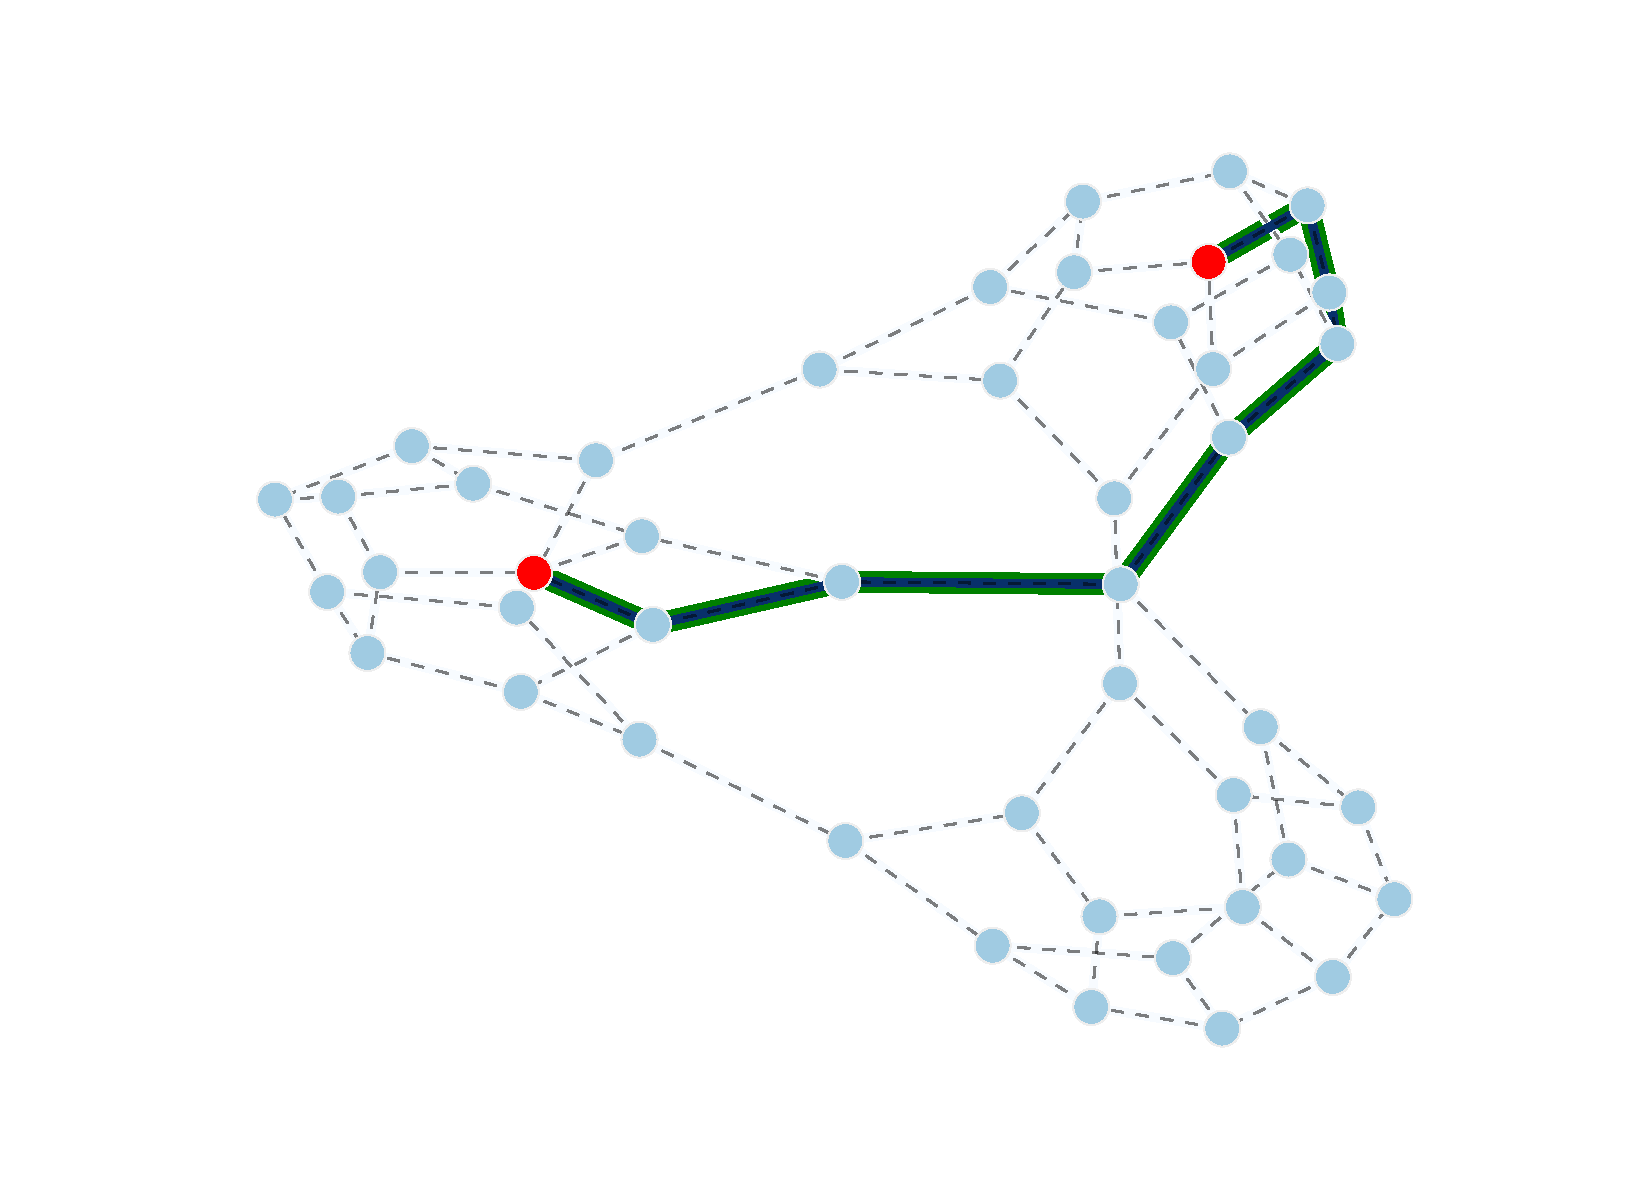
\includegraphics[scale =0.4] {images/section2/experimentb/pheromones_15_.pdf}
	\label{fig:subfig12}
}
%\caption[Optional caption for list of figures]{Caption of subfigures \subref{fig:subfig1}, \subref{fig:subfig2}}
\label{fig:fig1}
\end{figure}

\newpage
\subsubsection{Ant-like II, $k=50$}

\begin{figure}[ht]
\centering
\subfigure[Fitness evolution]{
	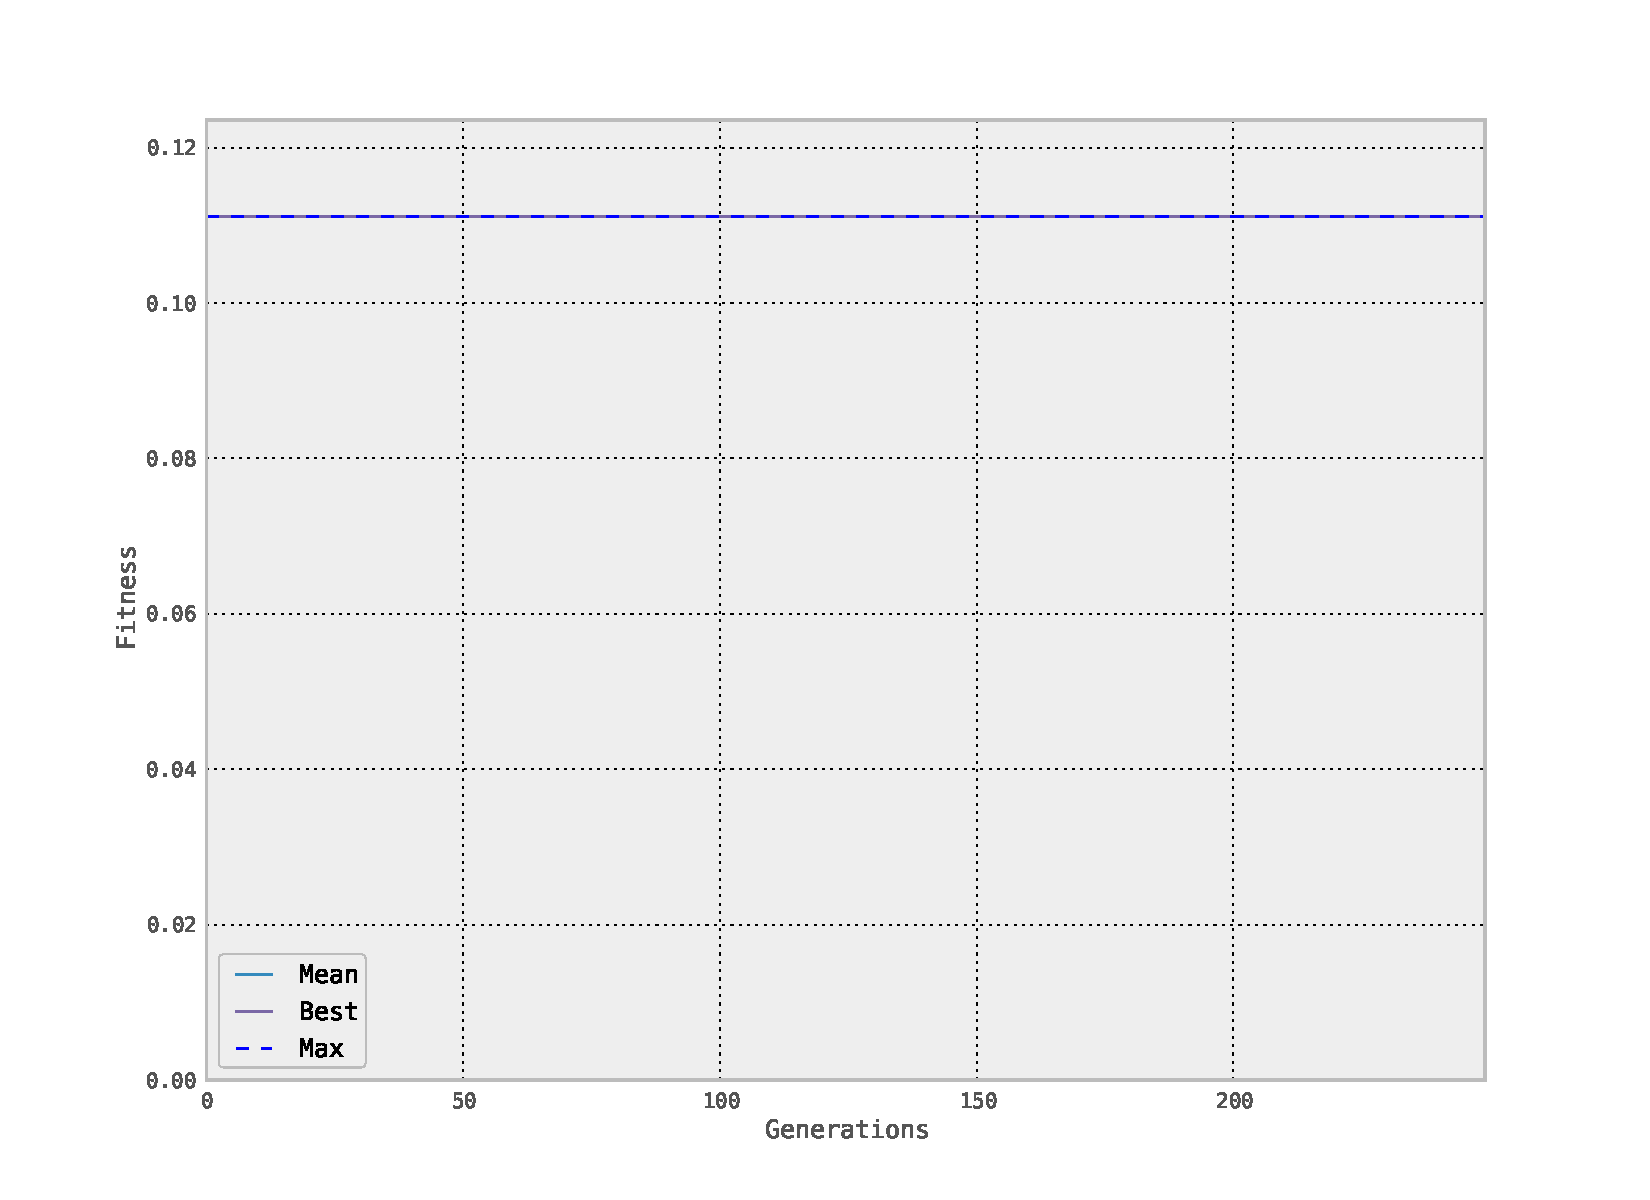
\includegraphics[scale =0.4] {images/section2/experimentb/fitness_50.pdf}
	\label{fig:subfig11}
}
\subfigure[Pheromones per edge]{
	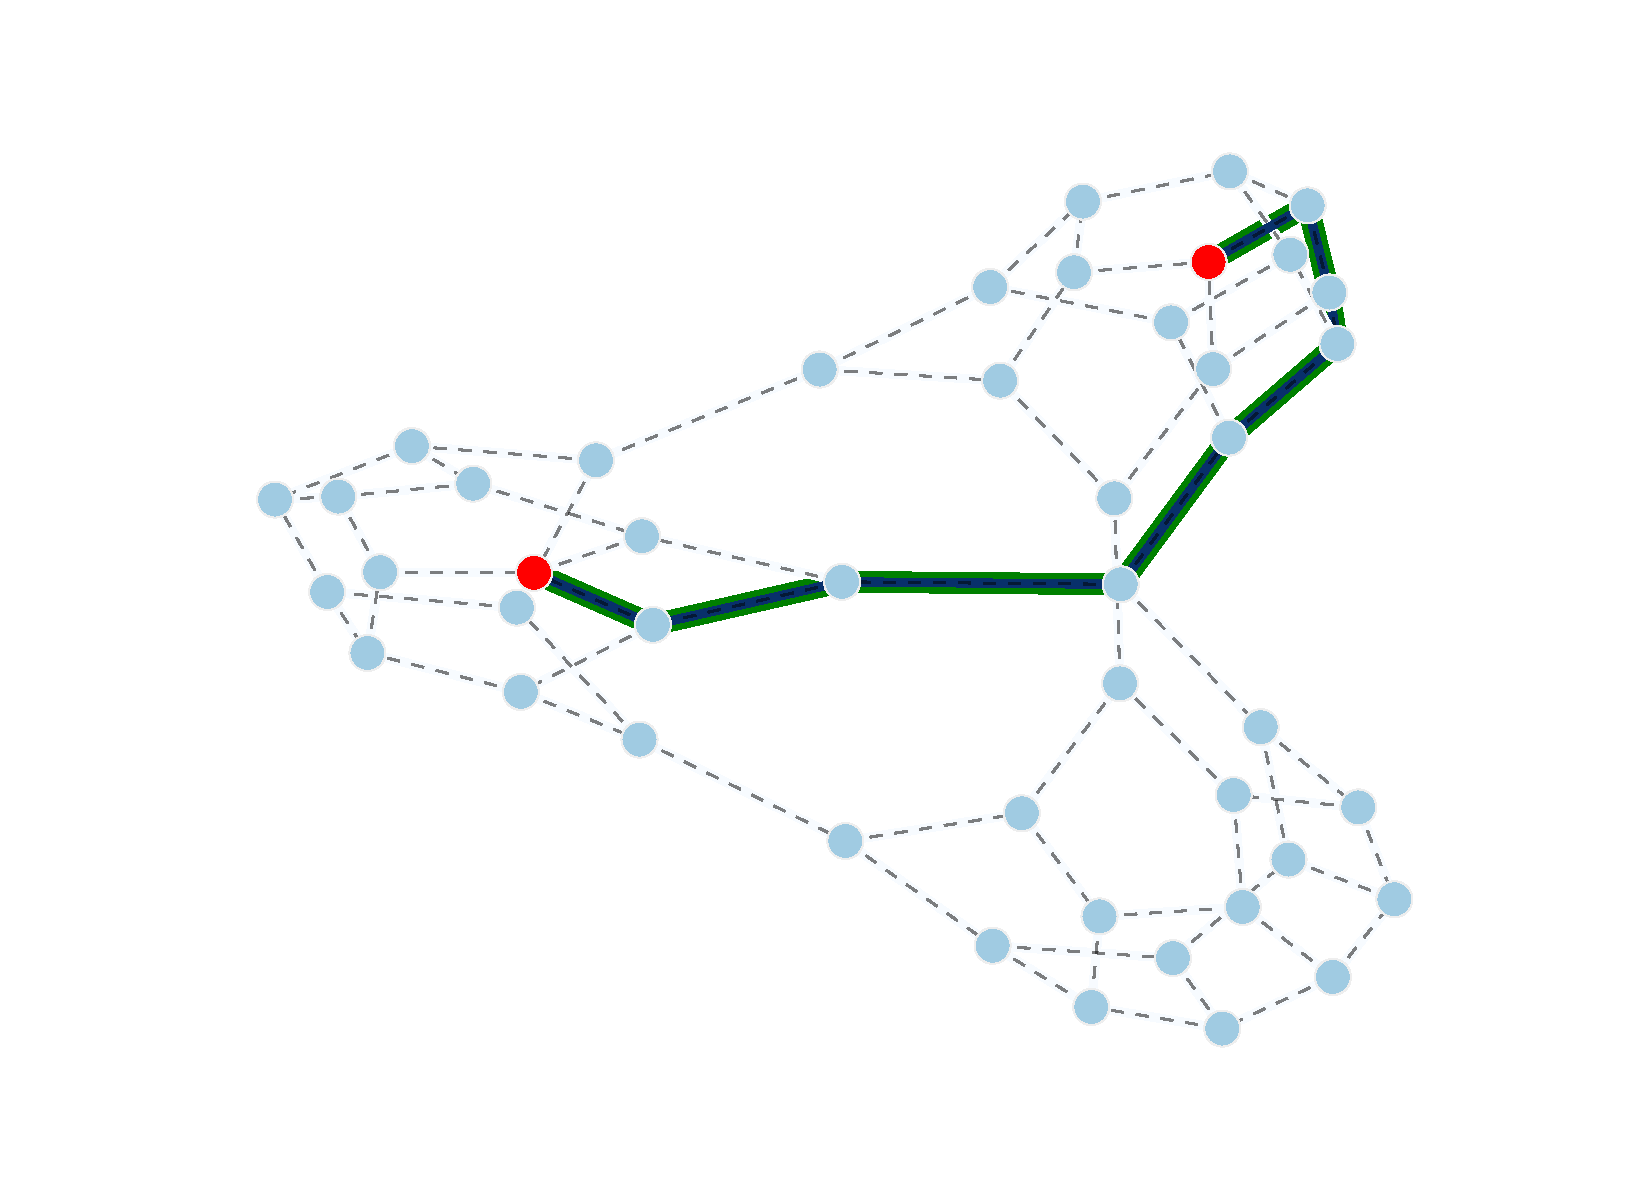
\includegraphics[scale =0.4] {images/section2/experimentb/pheromones_50_.pdf}
	\label{fig:subfig12}
}
%\caption[Optional caption for list of figures]{Caption of subfigures \subref{fig:subfig1}, \subref{fig:subfig2}}
\label{fig:fig1}
\end{figure}


\newpage
\subsubsection{Ant-like II, $k=100$}

\begin{figure}[ht]
\centering
\subfigure[Fitness evolution]{
	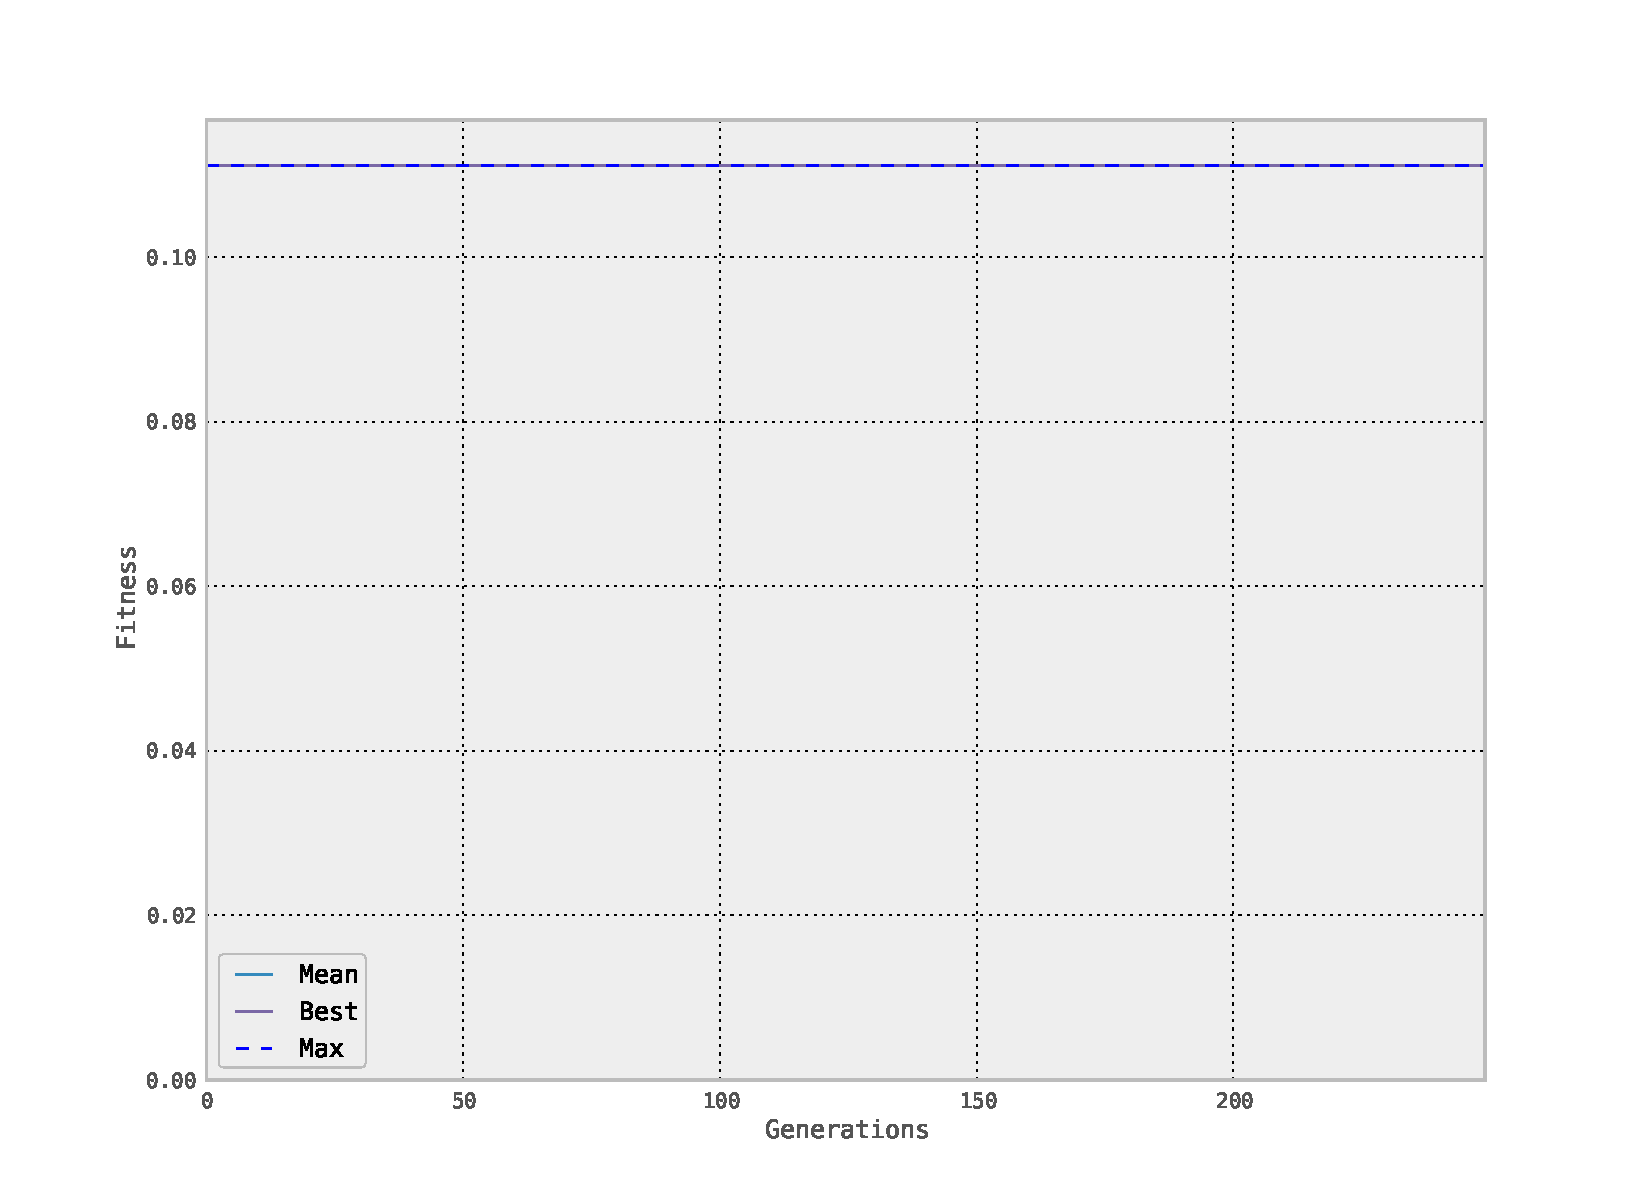
\includegraphics[scale =0.4] {images/section2/experimentb/fitness_100.pdf}
	\label{fig:subfig11}
}
\subfigure[Pheromones per edge]{
	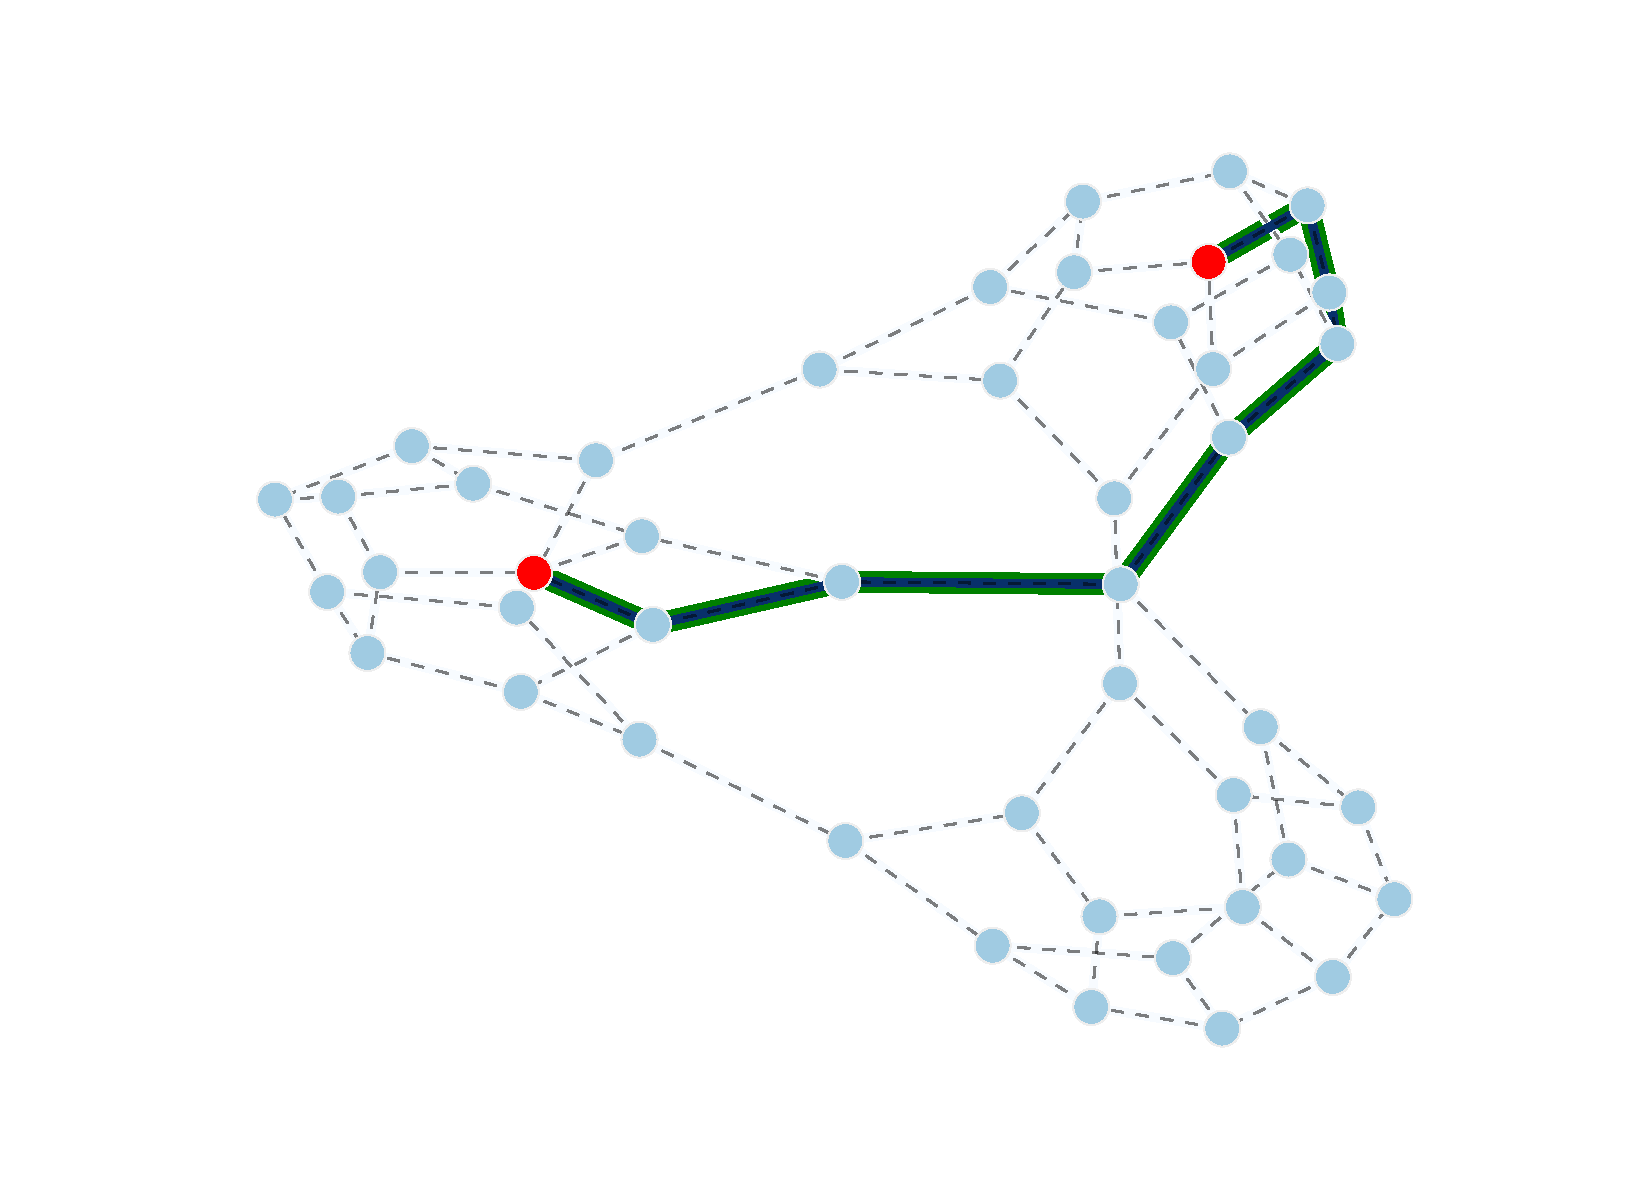
\includegraphics[scale =0.4] {images/section2/experimentb/pheromones_100_.pdf}
	\label{fig:subfig12}
}
%\caption[Optional caption for list of figures]{Caption of subfigures \subref{fig:subfig1}, \subref{fig:subfig2}}
\label{fig:fig1}
\end{figure}



\newpage
\subsection{Conclusions}
Ant-like I algorithm perform a better exploration, as we increase the variable $k$ from $5$ to $100$ the exploration decreases. Ant-like Ii algorithm always reach the best path, with $k=5$ we can get a suboptimal path near the optimal one, however, from $k=10$ to $k=100$ the best path is always reached.